In this section, we introduce Persistent Homology (PH), a foundational technique that played a pivotal role in the emergence of TDA, as developed by Carlsson, Edelsbrunner, Zomorodian, and others in the early 2000s~\cite{edelsbrunner2002topological, carlsson2004persistence, zomorodian2004computing}. PH captures the underlying shape patterns within complex data sets by studying the evolution of topological features across multiple scales.


 

\begin{wrapfigure}{r}{3in}
\vspace{-.1in}
    \centering
    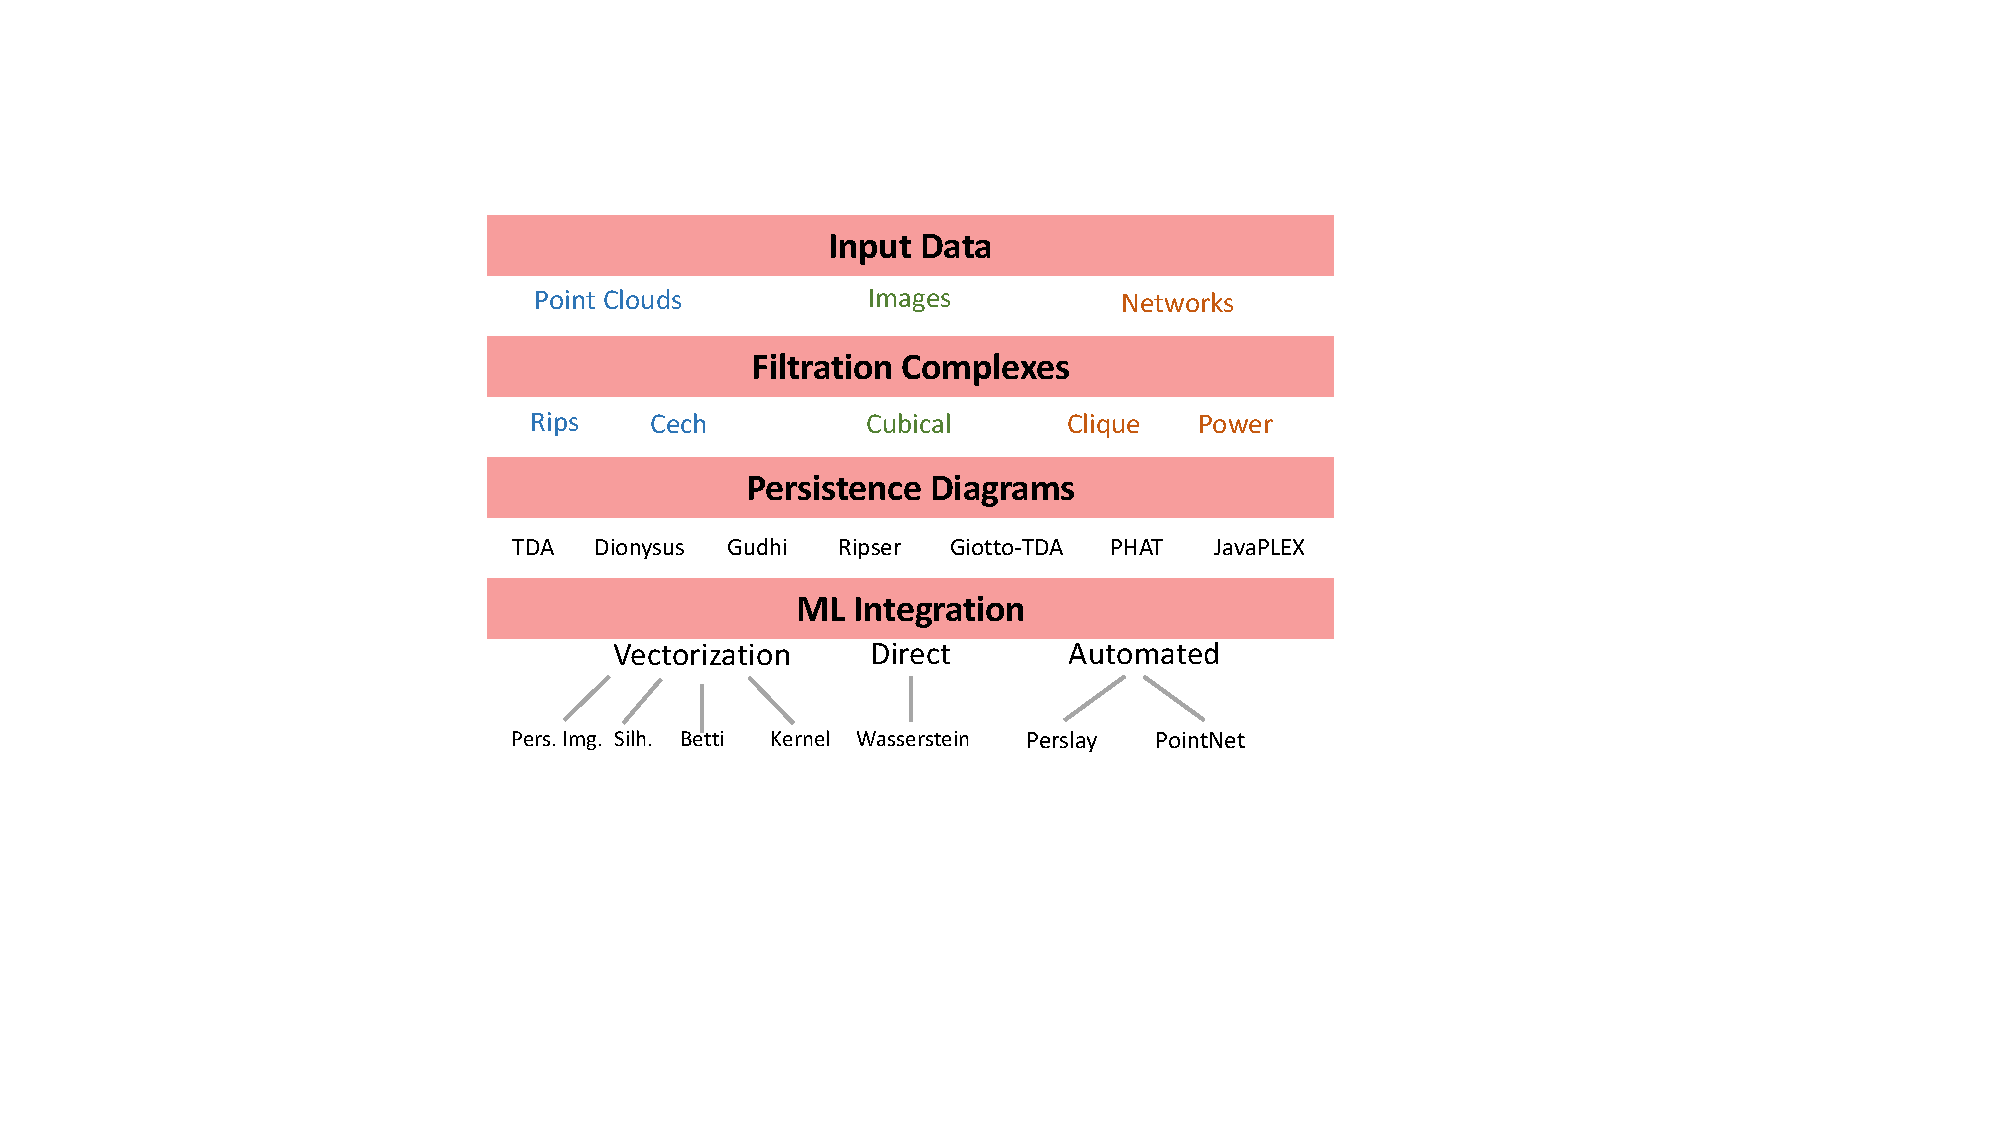
\includegraphics[width=\linewidth]{figures/PH_pipeline.pdf}
    \caption{\footnotesize \textbf{PH Pipeline.}  From data acquisition and filtration complex construction to generating persistence diagrams using software libraries. The final step highlights methods for integrating persistence diagrams into downstream ML tasks. \label{fig:pipe}}
    \vspace{-.15in}
\end{wrapfigure}
PH first constructs a nested sequence of simplicial complexes, known as \textit{filtration}, and tracks the birth and death of features, such as connected components, loops, and voids, in this sequence. The resulting multi-scale representation highlights significant features while filtering out noise, making PH a valuable tool in various fields, including medical imaging~\cite{singh2023topological}, biomedicine~\cite{skaf2022topological}, time series analysis~\cite{zeng2021topological}, material science~\cite{obayashi2022persistent}, geography~\cite{corcoran2023topological}, shape analysis~\cite{turkes2022effectiveness} and finance~\cite{ismail2022early}.

In the following, we explain PH in an accessible way, focusing on its key aspects relevant to ML applications. The main idea behind PH is to capture the hidden shape patterns in the data by using algebraic topology tools. PH achieves this by keeping track of the evolution of the topological features ($k$-holes, components, loops, and cavities) created in the data while looking at it in different resolutions.

In simple terms, PH can be summarized as a three-step procedure as follows.

\begin{enumerate}
    \item \textbf{Filtration}: Generate a  nested sequence of simplicial complexes derived from the data.
    \item \textbf{Persistence Diagrams}: Record the evolution of topological features across this sequence.
    \item \textbf{ML Integration}: Transform the persistence diagrams into vectors for efficient use in ML models.
\end{enumerate}


 

We provide details of these steps in the following sections. Although the second and third steps are conceptually similar across most settings, the first step, constructing filtrations, varies significantly depending on the data type, i.e., point clouds, images, and networks. See \Cref{fig:pipe} for a visual summary of PH pipeline.


 

 

\subsection{Constructing Filtrations} \label{sec:filtrations}

In \Cref{sec:background}, we introduced simplicial complexes which enable us to study the topological spaces via computational tools. To study the given data in different resolutions, PH generates a nested sequence of simplicial complexes $\K_1\subset \K_2\subset \dots \subset \K_n$ induced from the data. Such a sequence is called a {\em filtration}. This step can be considered the most crucial for the effectiveness of PH in ML applications. The primary reason is that the filtration process involves examining the data at different resolutions by adjusting a "scale parameter". The choice of this "scale parameter" can greatly influence the performance of the method.

For each data type, there are well-established methods to construct filtrations that have proven highly effective in their respective contexts. These methods vary significantly depending on the data type. While point cloud~\cite{chazal2015subsampling} and image~\cite{yadav2023histopathological} settings use relatively common approaches in their settings, the construction of filtrations in graph settings is notably more versatile~\cite{aktas2019persistence}.

\begin{wrapfigure}{r}{3in}
\vspace{-.15in}
    \centering
    \subfloat[$\epsilon=0.4$]{%
        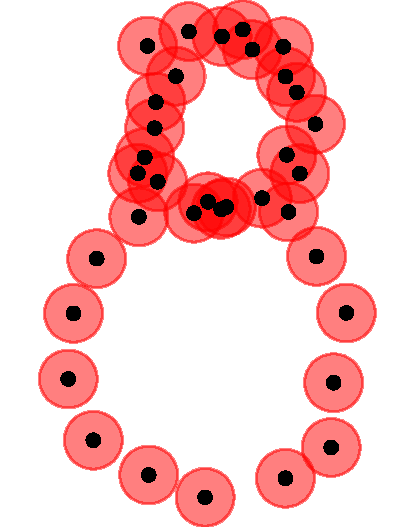
\includegraphics[width=0.33\linewidth]{figures/P8_0.4.pdf}
        \label{fig:p8_04a}
    }
    \subfloat[$\epsilon=0.7$]{%
        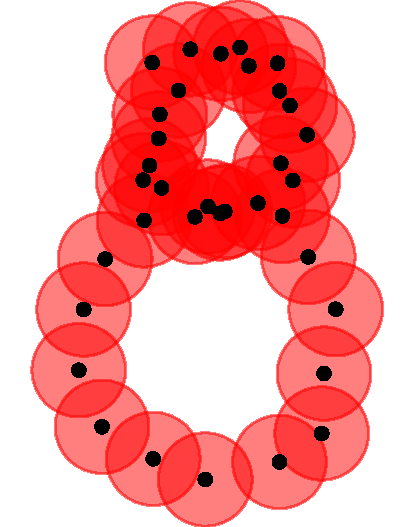
\includegraphics[width=0.33\linewidth]{figures/P8_0.7.pdf}
        \label{fig:p8_07a}
    }
    \subfloat[$\epsilon=2$]{%
        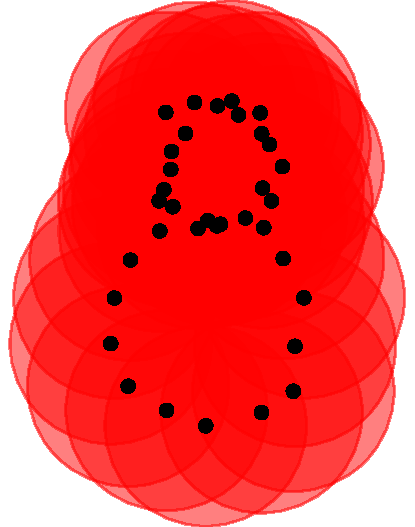
\includegraphics[width=0.33\linewidth]{figures/P8_2.pdf}
        \label{fig:p8_2a}
    }
    \caption{ For 8-shaped point cloud $\X$, $\{\N_\e(\X)\}$ filtration steps for thresholds $\e=0.4,\e=0.7$ an $\e=2$. \label{fig:point_filtration} }    
    \vspace{-.15in}
\end{wrapfigure}

\subsubsection{Filtrations for Point Clouds} \label{sec:point_cloud}
As the process is generally similar for various metric spaces, for simplicity, we will describe it for a point cloud $\X$ in $\mathbb{R}^N$ using the Euclidean metric. Let $\X = \{x_1, x_2, \dots, x_m\}$ be a point cloud in $\mathbb{R}^N$. We will define a nested sequence of simplicial complexes $\K_1 \subset \K_2 \subset \dots \subset \K_n$ induced by $\X$.  The central idea here is to build a series of simplicial complexes that progressively capture the topological picture of the point cloud $\X$ in different resolutions as we move from $\K_1$ to $\K_n$. The "nested" part signifies that each simplicial complex is contained within the next one, like a series of Russian Matryoshka dolls.

 


Before moving on to simplicial complexes, we will define a simpler nested sequence for $\X$. Let $\B_r(x)=\{y\in\R^N\mid d(x,y)\leq r\}$ be the closed $r$-ball around $x$. Then, let $r$-neighborhood of $\X$, $\N_r(\X) = \bigcup_{i=1}^m \B_r(x_i)$ be the union of $r$-balls around the points in $\X$. By declaring $r$ as our scale parameter, we first fix a monotone sequence of threshold values $0 = r_1 < r_2 < \dots < r_n$, where $r_n = \max_{i,j}\{d(x_i, x_j)\}$, the diameter of $\X$. These values intuitively represent the resolution at which we observe the point cloud $\X$. In particular, a smaller value of $r$ indicates a closer, more detailed examination of $\X$, while a larger value of $r$ means observing the point cloud with a broader view from a greater distance, making it difficult to distinguish between points that are close together in $\X$. This naturally gives a nested sequence of topological spaces $\N_{r_1}(\X) \subset \N_{r_2}(\X) \subset \dots \subset \N_{r_n}(\X)$ (See~\Cref{fig:point_filtration}). While these neighborhoods  $\{\N_r(\X)\}$ give a natural sequence for the data, to effectively leverage computational tools, we need to induce a \textit{sequence by simplicial complexes}. There are two common ways to achieve this while preserving the underlying topological information.






 
\begin{wrapfigure}{r}{3in}
\vspace{-.25in}
    \centering
    \subfloat[Cech Complex]{%
        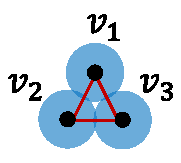
\includegraphics[width=0.33\linewidth]{figures/cech.pdf}
        \label{fig:cech}    }
       \subfloat[Rips Complex]{%
        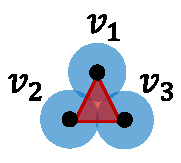
\includegraphics[width=0.33\linewidth]{figures/rips.pdf}
        \label{fig:rips}    }
        \subfloat[Cech Complex]{%
        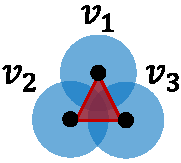
\includegraphics[width=0.33\linewidth]{figures/cech2.pdf}
        \label{fig:cech2}    }
    \caption{\footnotesize \textbf{Comparison of Rips and \v{C}ech Complexes.} In panels~\ref{fig:cech} and \ref{fig:rips}, the \v{C}ech and Rips complexes differ: the \v{C}ech complex does not form a 2-simplex among $v_1$, $v_2$, and $v_3$ due to insufficient ball overlap, while the Rips complex does. A larger radius, as in panel~\ref{fig:cech2}, is needed for the \v{C}ech complex to include this simplex.}
    \label{fig:ripsandcech}
    \vspace{-.25in}
\end{wrapfigure}

\paragraph*{Method 1 - Rips complexes:} For $\X\subset \R^N$, and for $r>0$, the \textit{Rips complex} (aka Vietoris-Rips complex) is the abstract simplicial complex $\VR_r(\X)$ where a $k$-simplex $\sigma=[x_{i_0},x_{i_1},\dots,x_{i_k}]\in \VR_r(\X)$
if and only if $d(x_{i_m},x_{i_n})< r$ for any $0\leq m,n\leq k$. In other words, for $r>0$, if for $k+1$-points are pairwise $r$-close to each other, they form a $k$-simplex in $\VR_r(\X)$. 


\paragraph*{Method 2 - \v{C}ech complexes:} Similarly,  for $\X\subset \R^N$, and for $r>0$, the \v{C}ech complex is the abstract simplicial complex $\check\C_r(\X)$ where a $k$-simplex $\sigma=[x_{i_0},x_{i_1},\dots,x_{i_k}]\in \check\C_r(\X)$ if and only if $\bigcap_{j=0}^k B_r(x_{i_j})\neq \emptyset$. Here, the condition to build $k$-simplex is different as we ask for a nontrivial intersection of the $r$-balls of the $k+1$-points. 


\begin{algorithm}[b]
\caption{PH Machinery for Point Clouds with Rips Complexes \label{alg:PH_point}}
\begin{algorithmic}[1]
\State \textbf{Input:} Point cloud $P$, Distance metric $d$, Threshold set $\{\epsilon_i\}_{i=0}^n$
\State \textbf{Output:} Topological vector $\vec{\beta}(P, d, \{\epsilon_i\})$
\State $V \gets \{v \in P\}$ \Comment{Vertex set doesn't change with filtration}
\For{$i = 0$ to $n$} \Comment{Filtration index}
    \State \textbf{Vertex set remains the same for all $i$}
    \State $E_i \gets \{(u, v) \mid u, v \in P \text{ and } d(u, v) \leq \epsilon_i\}$ \Comment{Edges with distance $\leq \epsilon_i$}
    \State $\VR_i \gets  (V, E_i)$ \Comment{Rips complex at $\epsilon_i$}
\EndFor
\For{$k = 0$ to $1$} \Comment{Topological dimensions}
    \State Compute persistence diagram $\mathrm{PD}_k(\{\VR_i\}_{i=0}^n)$
    \State Obtain vectorization $\vec{\beta}_k$ from $\mathrm{PD}_k(\{\VR_i\}_{i=0}^n)$
\EndFor
\State \textbf{Return} Concatenation of $\vec{\beta}_0$ and $\vec{\beta}_1$, denoted as $\vec{\beta}(P, d, \{\epsilon_i\}) = \vec{\beta}_0 \mathbin\Vert \vec{\beta}_1$
\end{algorithmic}
\end{algorithm}

 




The main relationship between our original filtration $\{\N_{r_i}(\X)\}$ and the simplicial complex filtrations arises from the \textit{Nerve Lemma}. This lemma states that the \v{C}ech complex $\check{\mathcal{C}}_r(\X)$ is homotopy equivalent to $\N_r(\X)$ for any $r \geq 0$~\cite{dey2022computational}. Since homotopy equivalent spaces have the same homology, we have $\h_k(\check{\mathcal{C}}_r(\X)) \simeq \h_k(\N_r(\X))$ for any $k \geq 0$. Therefore, from a PH perspective, the filtrations $\{\N_{r_i}(\X)\}_1^n$ and $\{\check{\mathcal{C}}_{r_i}(\X)\}_1^n$ are essentially the same. Furthermore, for $\X \subset \R^N$ with the Euclidean metric, Rips and \v{C}ech complexes are closely related and produce similar topological information as  $\check{\mathcal{C}}_r(\X) \subset \VR_{2r}(\X) \subset \check{\mathcal{C}}_{\sqrt{2}r}(\X)$~\cite{edelsbrunner2022computational}.

While both complexes provide similar filtrations, Rips complexes are more commonly used in practice. This preference is due to the fact that Rips complexes only require the pairwise distances $\{d(x_i, x_j)\}$ among points, which can be easily obtained at the beginning of the process. Hence, constructing Rips complexes is straightforward once these distances are known. In contrast, constructing \v{C}ech complexes requires checking whether collections of $r$-balls have nontrivial intersections. \Cref{fig:ripsandcech} depicts their differences in a toy scenario.

In particular, Rips complexes are the most common filtration type used for point clouds because of their computational practicality, and because of the Nerve Lemma, they capture very similar information produced by the simple neighborhood filtration $\{N_r(\X)\}$ described earlier.

Although we discuss the construction for point clouds in $\R^N$, the same process can be applied to any metric space (any space with a distance function). Furthermore, in some cases, the point cloud $\X$ is given in an abstract setting, where only pairwise distances $\{d(x_i, x_j)\}$ among the points are provided. The Rips complex filtration can be effectively applied to such point clouds. In~\Cref{sec:shape}, we detail the real-life application of this approach for shape recognition. 


\paragraph*{Other complex types.} One of the primary challenges in applying PH to point clouds is the computational cost. To mitigate this, \textit{witness complexes} offer a valuable alternative for efficiently analyzing the topological features of point clouds, especially in high-dimensional spaces. Unlike the Rips complexes, which can be computationally expensive, witness complexes reduce complexity by utilizing a \textit{representative subset} of the data points, known as \textit{witnesses}, to construct the simplicial complex~\cite{otter2017roadmap}. This method strikes a balance between computational efficiency and topological accuracy, making it particularly well-suited for large datasets where constructing full complexes would be impractical. By concentrating on representative data points (witnesses), witness complexes facilitate a more manageable and scalable computation of persistent homology, enabling the detection of the underlying shape and features of the point cloud across various scales. In addition to Rips and Čech complexes, other types of complexes, such as \textit{alpha complexes} and \textit{Delaunay complexes}, are particularly useful in lower-dimensional spaces. However, to maintain the focus of this paper, we refer the reader to~\cite{otter2017roadmap} for an in-depth discussion of these complexes.
 






\begin{figure}[t] 
\centering
    	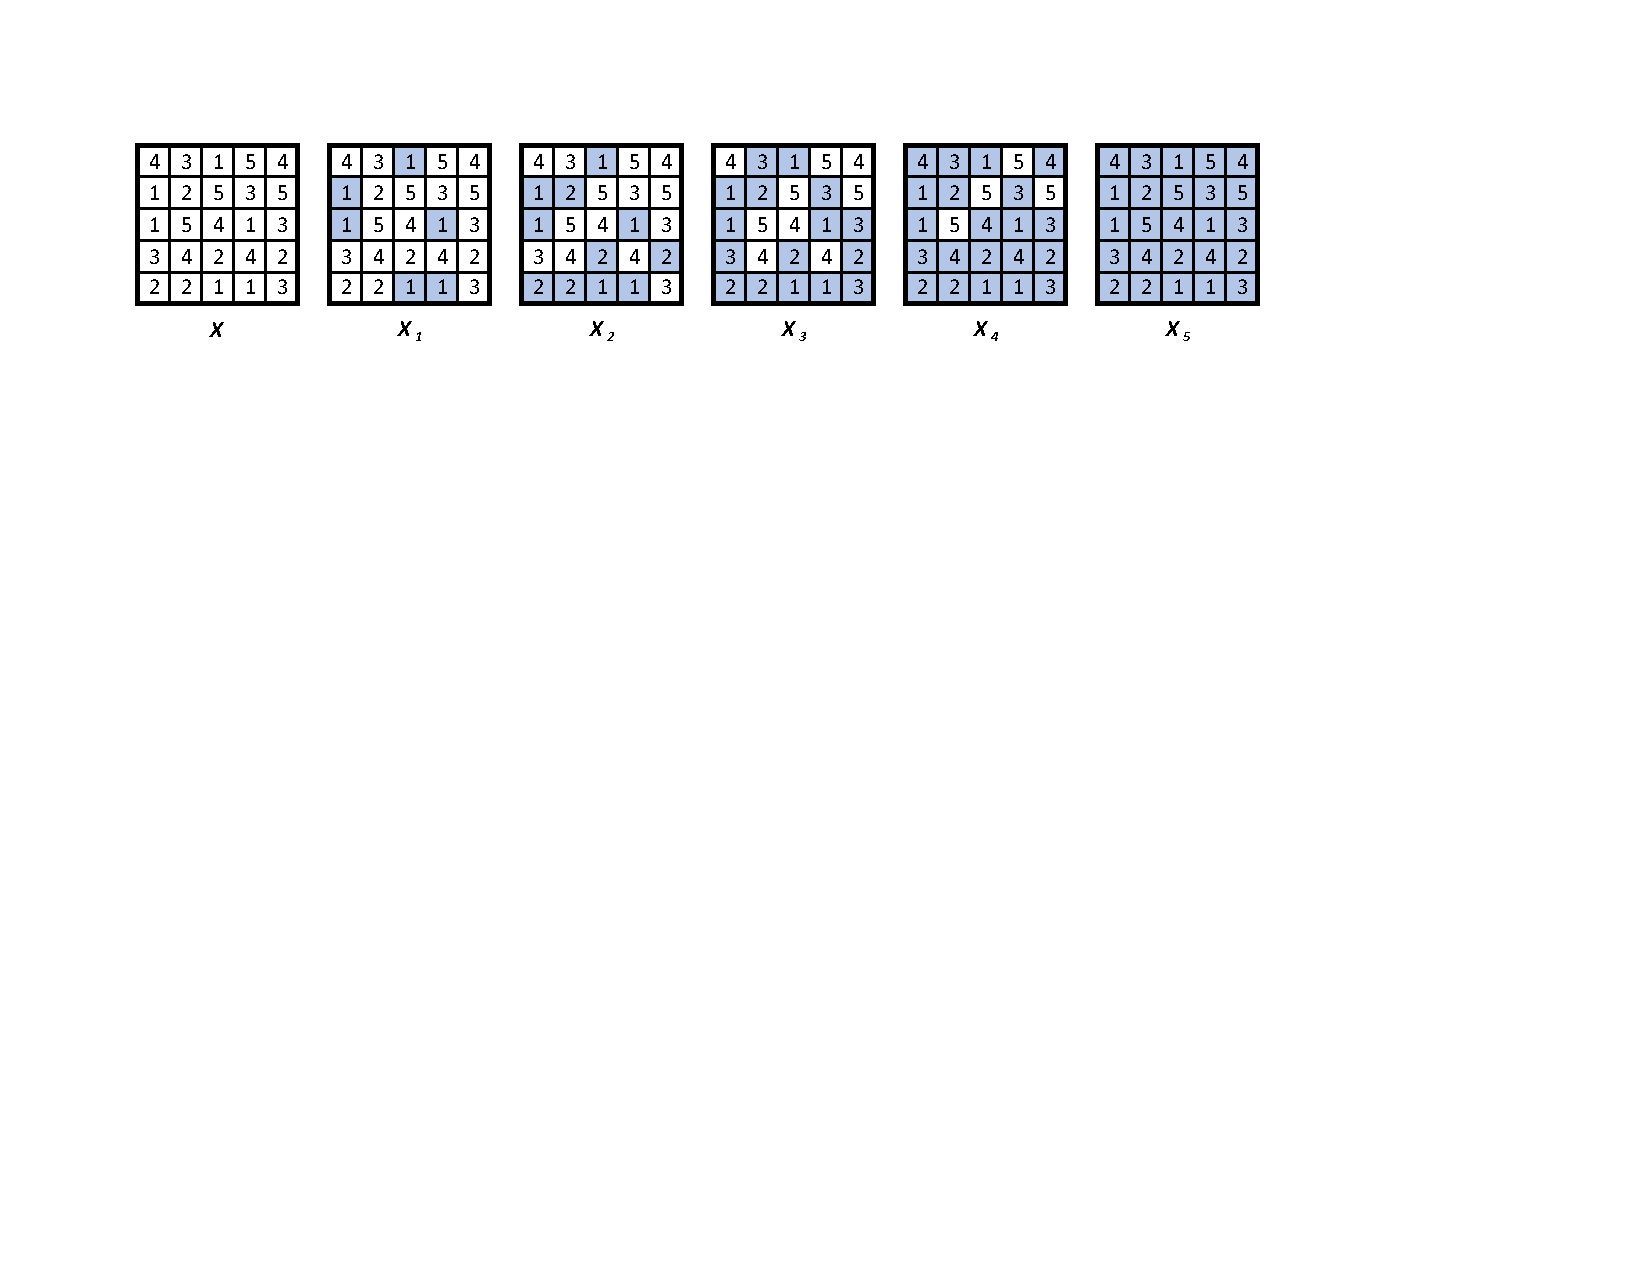
\includegraphics[width=\linewidth]{figures/filtration4.pdf}  
 {\caption{For the $5\times 5$ image $\X$ with the given pixel values, \textbf{the sublevel filtration} is the sequence of binary images $\X_1\subset \X_2\subset \X_3\subset \X_4\subset \X_5$. \label{fig:image-filtration}}}
   \vspace{-.2in}
    \end{figure}


\subsubsection{Filtrations for Images} \label{sec:image}

For images, constructing filtrations differs significantly due to the unique structure of image data. To keep the explanation simple, we will focus on 2D images, though the concepts can be extended to 3D and other types of images. Filtration for images typically involves nested sequences of binary images, known as \textit{cubical complexes}~\cite{kaji2020cubical}. Starting with a given color (or grayscale) image $\X$ of dimensions $r \times s$, we first select a specific color channel (e.g., red, blue, green, or grayscale). The color values $\gamma_{ij} \in [0, 255]$ of individual pixels $\Delta_{ij} \subset \X$ are used, where $\Delta_{ij}$ represents a \underline{closed box} (square including its boundary) in the $i^{th}$ row and $j^{th}$ column of the image $\X$.


\begin{figure}[b]
\vspace{-.2in}
    \centering
    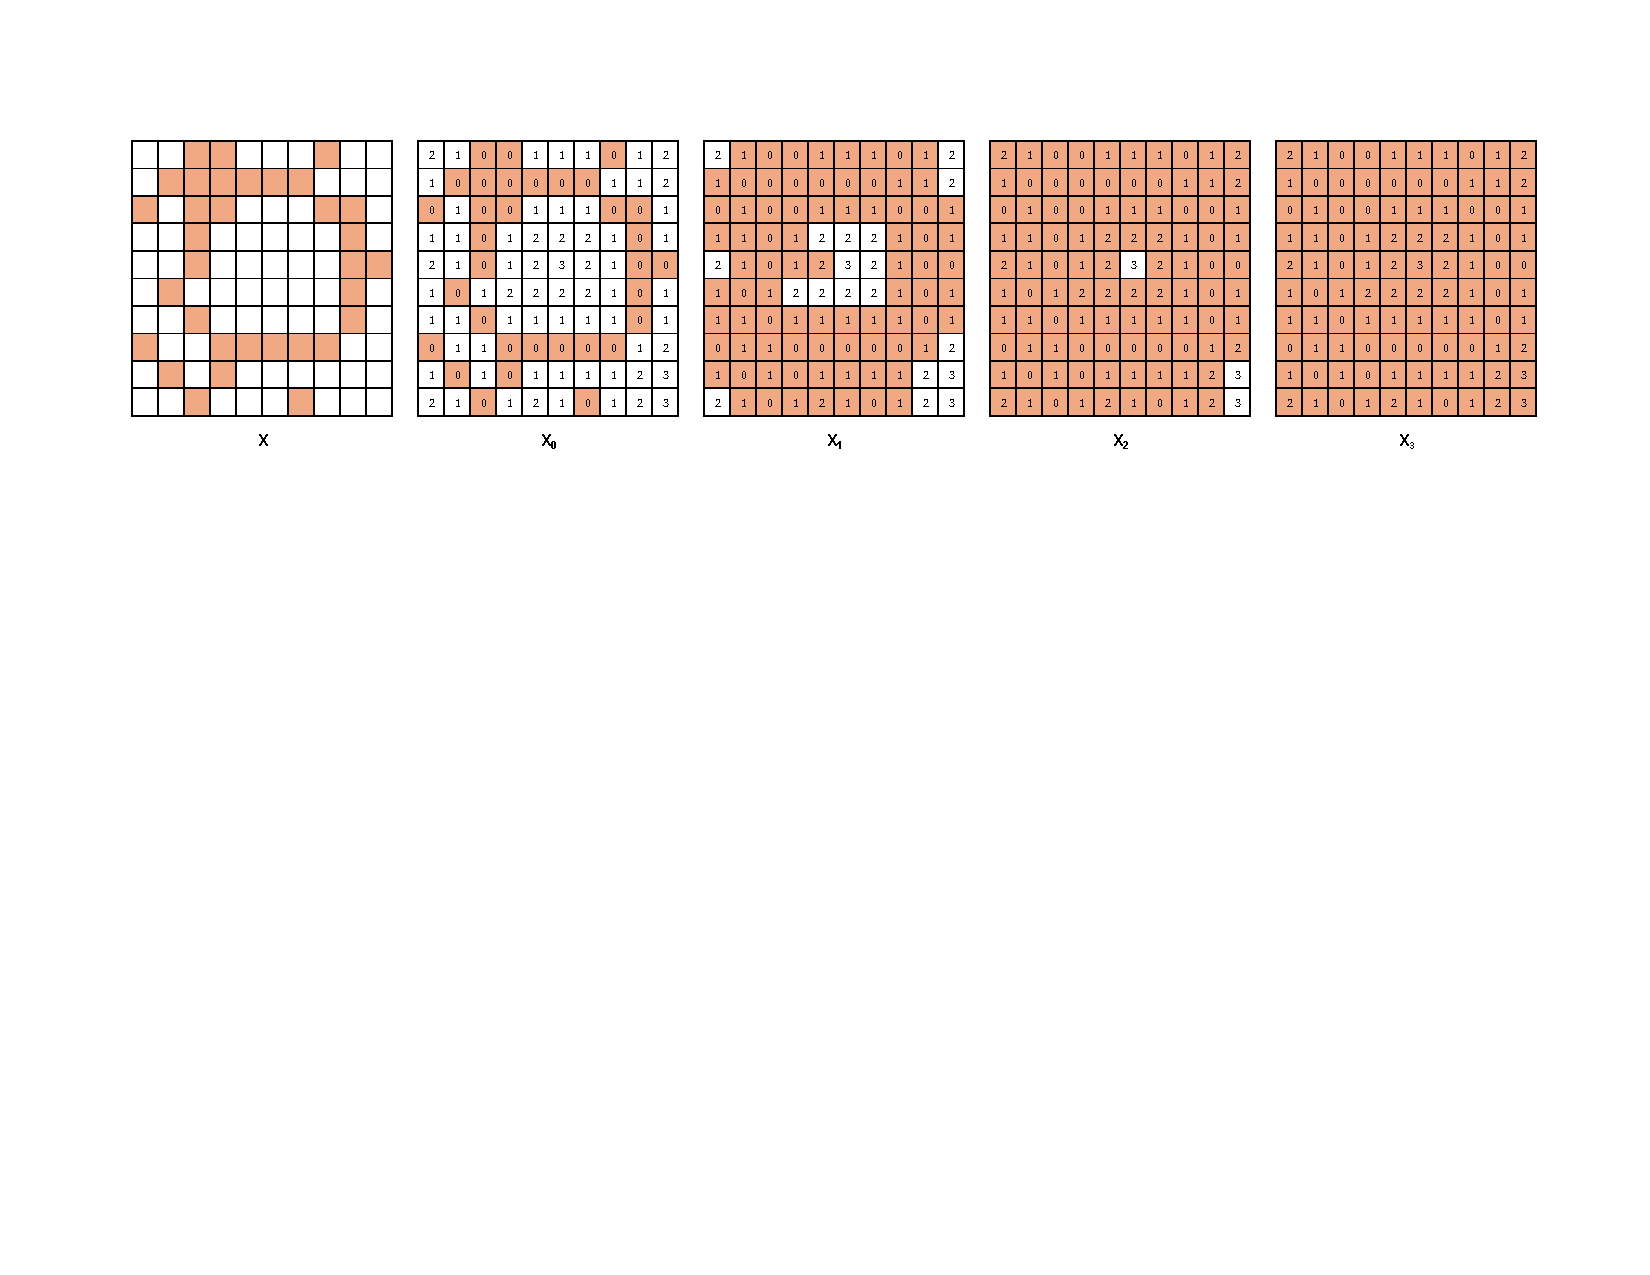
\includegraphics[width=\linewidth]{figures/erosion2.pdf}
    \caption{\footnotesize {\bf Erosion Filtration.} For a given binary image $\X$, we define the erosion function, which assigns a value of 0 to black pixels and the distance to the nearest black pixel for white pixels (shown in $\X_0$). From this, we generate a filtration of binary images, $\X_0 \subset \X_1 \subset \dots \subset \X_3$, where each $\X_i$ is obtained by activating pixels that reach a specific threshold value. \label{fig:erosion}}    
\end{figure}
Next, we choose the number  of thresholds "$n$" to span the color interval $[0, 255]$, i.e., $0 = t_1 < t_2 < \dots < t_n = 255$. This determines the length of our filtration sequence, with a typical range being between 50 and 100. Using these thresholds, we define a nested sequence of binary images (cubical complexes) $\X_1 \subset \X_2 \subset \dots \subset \X_n$ such that $\X_m = \{\Delta_{ij} \subset \X \mid \gamma_{ij} \leq t_m\}$ (see \Cref{fig:image-filtration}).

In particular, this involves starting with a blank $r \times s$ image and progressively activating (coloring black) pixels as their grayscale values reach each specified threshold $t_m$. This process is known as {\em sublevel filtration}, applied to $\X$ relative to the chosen color channel (in this case, grayscale). Alternatively, pixels can be activated in descending order, referred to as {\em superlevel filtration}. In this context, let $\Y_m = \{\Delta_{ij} \subset \X \mid \gamma_{ij} \geq s_m\}$, where $255 = s_1 > s_2 > \dots > s_n = 0$, and $\Y_1 \subset \Y_2 \subset \dots \subset \Y_n$ is called superlevel filtration. The persistence homology process involving such cubical complexes has a special name, called {\em cubical persistence}. In \Cref{sec:histo}, we detail a successful application of this method in cancer detection from histopathological images.

While these sublevel and superlevel filtrations are common choices for color or grayscale images, there are other filtration types used for binary images, e.g., erosion, dilation, and signed distance~\cite{garin2019topological}. These filtrations are specific to binary images and effective in capturing the size and other properties of topological features. In~\Cref{fig:erosion}, we give an example of erosion filtration.




\begin{algorithm}[t]
\caption{PH Machinery for Images with Cubical Persistence \label{alg:PH_image}}
\label{alg:cubical}
\begin{algorithmic}[1]
\State \textbf{Input:} Image $\mathcal{X}$, Color channel $F: \mathcal{X} \to \mathbb{R}$, Threshold set $\{\epsilon_i\}_{i=0}^n$
\State \textbf{Output:} Topological vector $\vec{\beta}(\mathcal{X}, F, \{\epsilon_i\})$
\For{$i = 0$ to $n$} \Comment{Filtration index}
    \State $\mathcal{X}_i \gets \{\Delta_{ij} \in \mathcal{X} \mid F(\Delta_{ij}) \leq \epsilon_i\}$ \Comment{Binary Images}
   % \State $\mathcal{K}_i \gets$ Cubical complex corresponding to $\mathcal{I}_i$
\EndFor
\For{$k = 0$ to $1$} \Comment{Topological dimensions}
    \State Compute persistence diagram $\mathrm{PD}_k(\{\mathcal{X}_i\}_{i=0}^n)$
    \State Obtain vectorization $\vec{\beta}_k$ from $\mathrm{PD}_k(\{\mathcal{X}_i\}_{i=0}^n)$
\EndFor
\State \textbf{Return} Concatenation of $\vec{\beta}_0$ and $\vec{\beta}_1$, denoted as $\vec{\beta}(\mathcal{X}, F, \{\epsilon_i\}) = \vec{\beta}_0 \mathbin\Vert \vec{\beta}_1$
\end{algorithmic}
\end{algorithm}











\subsubsection{Filtrations for Graphs} \label{sec:graph}

Graphs are a widely used application domain for PH because they generate highly effective features that are not easily obtained through other methods. While filtration methods for point clouds and images are relatively standard, graph filtrations offer a variety of choices. The way you construct these filtrations can significantly impact the performance of ML models. Unlike other data formats, there are various methods to construct filtrations from graphs, where the details can be found in~\cite{aktas2019persistence}. We categorize these methods into two groups:


\paragraph*{i. Filtrations through node/edge functions.} This type of filtration is computationally efficient in most cases and is commonly used in applications. The main concept involves defining a filtration function on nodes or edges and using the order dictated by these functions to create a sequence of subgraphs and corresponding simplicial complexes. 

\begin{wrapfigure}{r}{3in}
\vspace{-.15in}
\centering
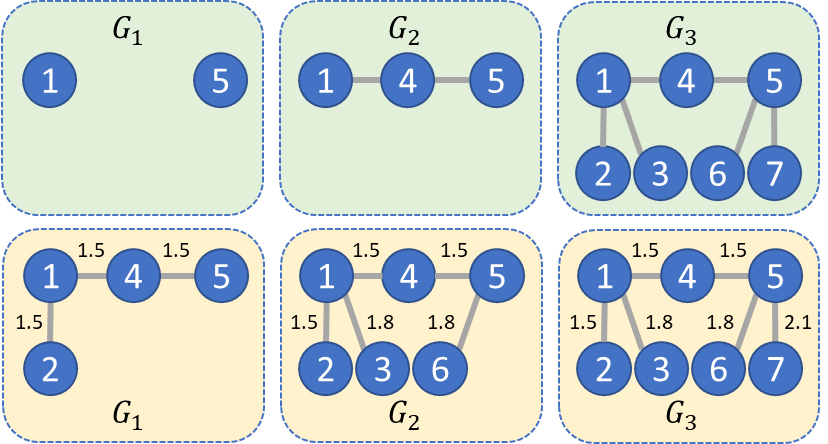
\includegraphics[width=\linewidth]{figures/graph-filtration.png}
\caption{\footnotesize \textbf{Graph Filtration.} For $\mathcal{G}=\mathcal{G}_3$ in both examples, the top figure illustrates a \textit{superlevel filtration using the node degree function} with thresholds $3>2>1$, where nodes of degree 3 are activated first, followed by those of lower degrees.  Similarly, the bottom figure illustrates a \textit{sublevel filtration based on edge weights} with thresholds $1.5< 1.8< 2.1$.  \label{fig:graph-filtration}}
\vspace{-.15in}
\end{wrapfigure}

Given a graph $\G=(\V,\E)$, let $f:\V\to\R$ be a \textit{node filtration function}. Common examples of such functions include degree, centrality, betweenness, closeness, and heat kernel signatures (HKS). Additionally, functions may be derived from the domain of the graph, such as atomic number for molecular graphs or account balance for transaction networks. These functions establish a hierarchy among the nodes, ordering them from less important to more important within the graph within the context defined by the filtration function.


To define the resolution of our filtration, we choose a set of thresholds that cover the range of $f$, denoted as $\mathcal{I}=\{\epsilon_i\}_1^n$, where $\epsilon_1=\min_{v \in \V} f(v) < \epsilon_2 < \ldots < \epsilon_n = \max_{v \in \V} f(v)$. For each threshold $\epsilon_i \in \mathcal{I}$, let $\V_i = \{v \in \V \mid f(v) \leq \epsilon_i\}$. Define $\G_i$ as the subgraph of $\G$ induced by $\V_i$, i.e., $\G_i = (\V_i, \E_i)$ where $\E_i = \{e_{ij} \in \E \mid v_i, v_j \in \V_i\}$. In other words, at each threshold, we activate the nodes whose values reach that threshold, along with the edges in the graph between these activated nodes.


This process results in a nested sequence of subgraphs $\G_1 \subset \G_2 \subset \ldots \subset \G_n = \G$ (See~\Cref{fig:graph-filtration}). For each $\G_i$, we define an abstract simplicial complex $\widehat{\G}_i$ for $1 \leq i \leq n$, creating a \textit{filtration} of simplicial complexes $\widehat{\G}_1 \subseteq \widehat{\G}_2 \subseteq \ldots \subseteq \widehat{\G}_n$. Typically, \textit{clique complexes} are used, where the complex $\widehat{\G}$ is obtained by assigning a $k$-simplex to each $(k+1)$-complete subgraph ($(k+1)$-clique) in $\G$~\cite{aktas2019persistence}. The term \textit{clique} refers to a group (clique) of $k+1$ vertices forming a $k$-simplex.  This is called {\em sublevel filtration} for the filtration function $f$. Similarly, one can reverse this process (using a decreasing order for activation of the nodes) to obtain a \textit{superlevel filtration}, where $\V_i = \{v \in \V \mid f(v) \geq \epsilon_i'\}$ where $\{\e_i'\}$ is a monotone decreasing sequence. %\textN{Bunu yapma nedenini anliyorum ama okuyucuyu gereksiz yere zorlar. Sonucta i thresholdlardan biri.}

While we have explained the process for node filtration functions, edge filtration functions are also common. This approach is frequently employed in weighted graphs or graphs with key edge functions for downstream tasks. For a graph $\G$, let $g: \E \to \R$ be an \textit{edge filtration function}. In the case of weighted graphs, the weight function $w: \E \to \R$ with $w(e_{ij}) = \omega_{ij}$ serves as an example of such a function. Other common examples include Forman Ricci and Ollivier Ricci curvatures, which assign the (weighted or unweighted) edge a curvature value by interpreting the geometry of the edge's neighborhood~\cite{fesser2024augmentations}. Furthermore, edge filtration functions can be derived from the graph's domain, such as transaction amounts in blockchain networks~\cite{abay2019chainnet} or density in traffic networks~\cite{carmody2021topological}. These functions establish a hierarchy among the edges, similar to node filtration functions.

  

Again, by choosing the threshold set $\mathcal{I}=\{\e_i\}_{i=1}^n$ with $\e_1=\min_{e_{ij}\in\E}g(e_{ij})<\e_2<\ldots<\e_n=\max_{e_{jk}\in\E}g(e_{jk})$, we define the filtration as follows. For $\e_i\in \mathcal{I}$, let $\mathcal{E}_i=\{e_{jk}\in\mathcal{E}\mid g(e_{jk})\leq \e_i\}$. %\textN{$\omega$ degil de $g(e_{jk})$ kullanmak gerekiyor sanirim}. 
Let $\mathcal{G}_i$ be a subgraph of $\mathcal{G}$ induced by $\mathcal{E}_i$, i.e., $\mathcal{G}_i$ is the smallest subgraph of $\mathcal{G}$ containing the edge set $\mathcal{E}_i$ (Fig. \ref{fig:graph-filtration}). In other words, for each threshold, we activate the edges whose value reaches that threshold, along with the nodes attached to them. Again, this induces a nested sequence of subgraphs $\mathcal{G}_1\subset  \dots\subset\mathcal{G}_n=\mathcal{G}$. Then, one can follow the same steps by using clique complexes as before. 

In \Cref{fig:graph-filtration}, we give a toy example for superlevel (node) and sublevel (weight) filtrations. Here, we list the most common node and edge filtration functions used in applications:

\begin{itemize}
    \item {\em Node Filtration Functions:} Degree, betweenness, centrality, eccentricity, heat kernel signature (HKS), Fiedler values (spectral), node functions from the domain of the data.
    \item {\em Edge Filtration Functions:} edge weights (weighted graphs), Ollivier Ricci, Forman Ricci curvature, 
\end{itemize}




\begin{algorithm}[t]
\caption{PH machinery for graphs (sublevel filtration) \label{alg:PH_graph}}

\begin{algorithmic}
\State \textbf{Input:} Graph $\mathcal{G} = (\mathcal{V}, \mathcal{E})$, Filtration function $f: \mathcal{V} \to \mathbb{R}$, Threshold set $\mathcal{I} = \{\epsilon_i\}_{i=0}^n$
\State \textbf{Output:} Topological vector $\vec{\beta}(\mathcal{G}, f, \mathcal{I})$
%\State Initialize lists $\vec{\beta}_0 \gets []$, $\vec{\beta}_1 \gets []$
\For{$i = 0$ to $n$} \Comment{Filtration index}
    \State $\mathcal{V}_i \gets \{v \in \mathcal{V} \mid f(v) \leq \epsilon_i\}$ \Comment{Vertex set changes with i}
    \State $\mathcal{G}_i \gets$ Induced subgraph of $\mathcal{G}$ with vertex set $\mathcal{V}_i$
    \State $\wh{\mathcal{G}}_i \gets$ Clique complex of $\mathcal{G}_i$
\EndFor
\For{$k = 0$ to $1$} \Comment{Topological dimensions}
    \State Compute persistence diagram $\mathrm{PD}_k(\{\wh{\mathcal{G}}_i\}_{i=0}^n)$
    \State Obtain vectorization $\vec{\beta}_k$ from $\mathrm{PD}_k(\{\wh{\mathcal{G}}_i\}_{i=0}^n)$
\EndFor
\State \textbf{Return} Concatenation of $\vec{\beta}_0$ and $\vec{\beta}_1$, denoted as $\vec{\beta}(\mathcal{G}, f, \mathcal{I}) = \vec{\beta}_0 \mathbin\Vert \vec{\beta}_1$
\end{algorithmic}
\end{algorithm}

 


\paragraph*{ii. Graph distance-based filtrations.} Next to the sublevel filtrations above, a completely distinct filtration method for graphs uses the distances between nodes. Essentially, it treats the graph as a point cloud, where pairwise distances between nodes are defined by graph distance, and applies Rips filtration (\Cref{sec:point_cloud}) to this point cloud. While this method is more computationally intensive than filtrations via node or edge functions, it can be highly effective for small graphs as it captures distance information and finer topological details.


To apply this method, we need to define graph distances between nodes. In an unweighted graph $\G = (\V, \E)$, a common approach is to set the distance between adjacent nodes to 1 ($\|e_{ij}\| = 1$) and define the distance between $v_i$ and $v_k$ as the length of the shortest path $\tau_{ik}$ in $\G$ with endpoints $v_i$ and $v_k$, i.e. $d(v_i, v_k) = \min \|\tau_{ik}\|$. Thus, each pairwise distance is an integer representing the number of hops needed to travel from $v_i$ to $v_j$ in $\G$. The largest such distance is the diameter of $\G$, denoted as $n$.

After obtaining the pairwise distances $\{d(v_i, v_j)\}$ between the nodes, we treat the graph as a point cloud $\V = \{v_1, v_2, \dots, v_m\}$ with these distances. Since all distances are integers, we use integer thresholds $\{r_i = i\}$ for $0 \leq i \leq n = \text{diam}(\G)$. Now, we are ready to define our filtration. For the filtration index, we use superscripts instead of subscripts, where the reason will become clear later. 




To make the exposition simpler, let $\wh{\G}^k$ be the Rips complex corresponding to $r=k$, and let $\G^k$ be the graph corresponding to the $1$-skeleton of $\wh{\G}^k$. Here $1$-skeleton means the graph itself with its nodes and edges, without considering any higher-dimensional elements like faces or solids that might be part of a more complex simplicial structure. For the distance parameter $r = 0$, we have $\wh{\G}^0 = \V$ since there are no edges in the Rips complex. It is easy to see that at the distance threshold of 1, $\mathcal{G}^1 = \mathcal{G}$ because all edges are automatically included in the complex when $r = 1$. Recall that $\wh{\G}^1$ is a Rips complex, hence any complete $j$-subgraph in $\G^1$ generates a $(j-1)$-simplex ($j$-clique) in the Rips complex $\wh{\G}^1$. In particular, $\wh{\G}^k$ is nothing but the clique (or flag) complex of $\G^k$. Furthermore, $\G^k$ is the graph with node set $\V$, and edge set $\E^k = \{e_{ij} \mid d(v_i, v_j) \leq k\}$, i.e., $\G^k=(\V,\E^k)$. Therefore, in the filtration $\wh{\G}^0 \subset \wh{\G}^1 \subset \dots \subset \wh{\G}^n$, all simplicial complexes have the same node set, but at each step, we add new edges and cliques. Finally, for $\wh{\G}^n$, the 1-skeleton is a complete graph with $m$ nodes, and hence the corresponding simplicial complex $\wh{\G}^n$ would be an $(m-1)$-simplex. 

\begin{wrapfigure}{r}{3in}
\centering
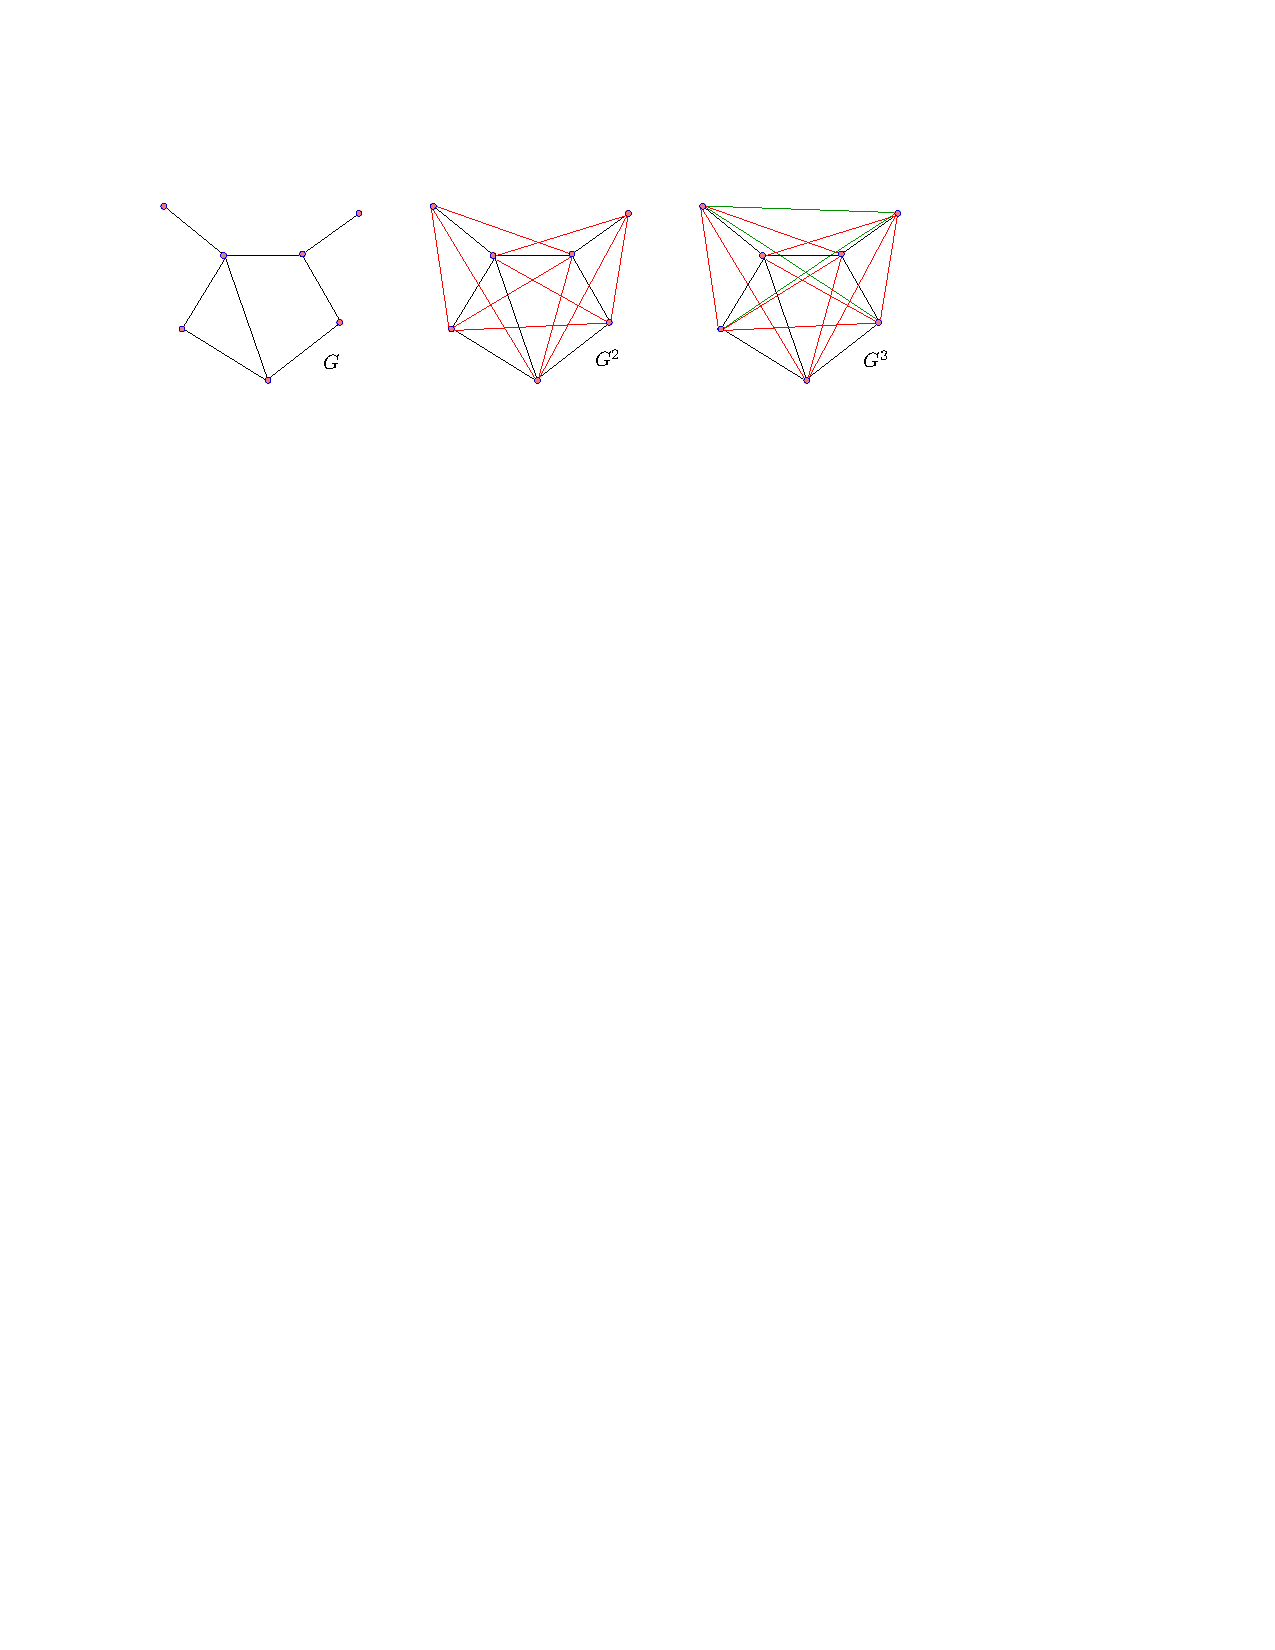
\includegraphics[width=\linewidth]{figures/power_filtration.pdf}
\caption{\footnotesize {\bf Graph Powers.} A graph $G=G^1$ and its graph powers.
	Red edges are added in $G^2$, and green ones are added in $G^3$.
	Note $\mathcal{G}^3$ is the complete graph on $7$ vertices since $D=\text{diam}(G)=3$. Hence, $\mathcal{G}^3$ would be a complete graph $\mathcal{K}_7$, and all higher powers are the same, i.e.\ $\mathcal{G}^n=\mathcal{G}^3$ for $n\geq 3$. \label{fig:power-filtration}} 
\end{wrapfigure}
The graphs $\{\G^k\}$ are called {\em graph powers} (See~\Cref{fig:power-filtration}), and this filtration is called the {\em power filtration} (or Rips filtration), hence the superscripts. Observe that the power filtration calculates the distances between every pair of vertices in the graph. Therefore, even vertices that are not direct neighbors or appear distant in the graph can still form a simplex in the later stages of the filtration. Note that you don't need to complete the entire filtration. In most cases, the critical insights information lies in the first few steps (e.g., up to $\e=5$ or $10$) for the power filtration. Given the high computational cost, it's both practical and reasonable to stop early.
 

For a weighted graph $\G = (\V, \E, \W)$, edge {lengths} can be defined using weights $\{\omega_{ij}\}$, where $\|e_{ij}\| = f(\omega_{ij})$ instead of the uniform $\|e_{ij}\| = 1$ used in unweighted graphs. The function $f: \W \to \R^+$ assigns distances based on weights, where a smaller $f(\omega_{ij})$ indicates that nodes $v_i$ and $v_j$ are closely related, and a larger distance indicates they are less related. This approach is particularly useful in financial networks where large edge weights (i.e., amounts) indicate stronger financial connections or dependencies. In~\Cref{sec:crypto}, we elaborate on this method in the context of a real-world application: Crypto-token anomaly forecasting.

Once edge lengths are defined, pairwise distances between any node pair can be calculated as the length of the shortest path as before, i.e., $d(v_i, v_j) = \min \|\epsilon_{ij}\|$, where $\epsilon_{ij}$ is any  such path in the graph with endpoints $v_i$ and $v_j$. After obtaining pairwise distances, the process is the same as for unweighted graphs.


\begin{wrapfigure}{r}{2in}
\vspace{-.1in}
    \centering
    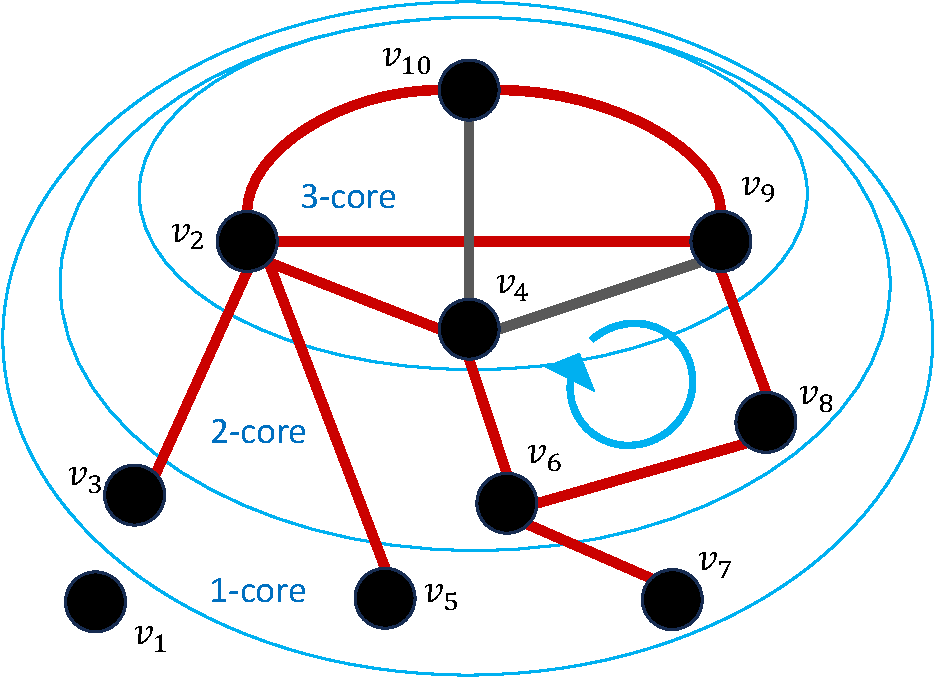
\includegraphics[width=\linewidth]{figures/kcore.pdf}
    \caption{{\bf Coral Reduction.} With CoralTDA, $2$-core of $\G$ has the same persistence diagrams $\PD_k(\G)$ for $k\geq 1$.}
    \label{fig:coraltrick}
    \vspace{-.1in} 
\end{wrapfigure}

\paragraph*{Graph Reduction and PH} Although PH generates highly effective topological embeddings for graph representation learning, scalability remains a challenge. To address this issue, Akcora et al.~\cite{akcora2022reduction} introduced two key methods to significantly reduce the computational costs of the PH process. The first method, \textit{CoralTDA}, leverages the observation that nodes with low graph-core do not contribute to persistence diagrams in higher dimensions. Specifically, they demonstrate that the $(k+1)$-core of a graph, which is a subgraph where each vertex has at least $k$ neighbors, is sufficient to compute the $\PD_k(\G)$ of the original graph. This improvement can be implemented as few as three lines of Python code (see the repository).  The second algorithm, \textit{PrunIT}, introduces an efficient method to reduce the size of graphs without altering their persistence diagrams. In this approach, a vertex \( u \) is said to dominate another vertex \( v \) if the $1$-neighborhood of $u$ contains $1$-neighborhood of $v$, i.e., $\N(u)\supset \N(v)$. The authors show that removing (pruning) a dominated vertex from the graph does not affect the persistence diagrams at any level as long as the dominated vertex enters the filtration after the dominating vertex.


\paragraph*{Which filtration to use for graphs?} We first note that filtrations using node/edge functions and filtrations based on graph distances are entirely different methods, producing distinct outputs. Distance-based filtrations are computationally demanding, but for datasets with small graphs (such as molecular graph datasets), power filtrations can be highly effective. Conversely, for larger graphs, the computational costs necessitate the use of filtration functions. In these cases, the choice of filtration function could be critical for performance~\cite{cai2020understanding}. Typically, relevant node or edge functions specific to the domain of the data are the best choices. If such functions are unavailable, heat kernel signatures (HKS) for node functions and Ollivier Ricci for edge functions are excellent alternatives. Choosing a filtration function can be seen as an outdated method, as letting ML algorithms select or construct the best filtration function for optimal performance is more reasonable. However, in many settings, model interpretability or greater control over the process is needed. In these instances, selecting a relevant filtration function is more suitable for the model.

If the goal is to achieve optimal performance with PH machinery, learnable filtration functions are a promising alternative. There are significant works, along with available code, that can be adapted for various tasks in graph representation learning~\cite{hofer2020graph,zhang2022gefl}.


\subsubsection{Choosing Thresholds} \label{sec:threshold} One of the key steps in effectively applying PH to ML problems is selecting the thresholds $\{\e_i\}_{i=1}^m$ for constructing the filtration. The first decision involves determining the number of thresholds, i.e., $m$. This number can be viewed as \textit{the resolution of the filtration}: a larger $m$ implies higher resolution, while a smaller $m$ indicates lower resolution. Then, a natural question arises: is there any disadvantage to choosing a large $m$? The answer is "Yes". Firstly, the computational cost increases with $m$. Secondly, the key information captured in the data may become diluted in higher dimensions, depending on the vectorization step. 

For graph filtrations, depending on the filtration function, selecting $m$ between 10 and 20 generally yields good results. Once the number of thresholds is set, they can be chosen equally spaced if the filtration function $f: \V \to \R$ (or $g: \E \to \R)$ is appropriate. Another effective method is to examine the distribution of the value set $\{f(v_i)\}$ for all vertices in the graphs across the dataset (or a random subsample), and then select the thresholds as the corresponding quantiles in this distribution. Similarly, for distance-based filtrations, analyzing the distribution of pairwise distances between vertices in a random subsample of the dataset can provide valuable insights for selecting appropriate thresholds.



For sublevel filtrations in the image setting, it’s important to choose thresholds that cover the color range $[0,255]$. Typically, using 50-100 thresholds yields good results. However, if the task only concerns a specific color interval $[a,b]$, it’s advisable to concentrate most or all thresholds within that range. These thresholds don't need to be evenly spaced. In the case of binary image filtrations (e.g., erosion, height, signed distance), thresholds are usually evenly distributed up to the maximum value.


\begin{wrapfigure}{r}{2.8in}
\vspace{-.25in}
    \centering
    \subfloat[$\epsilon=0.4$]{%
        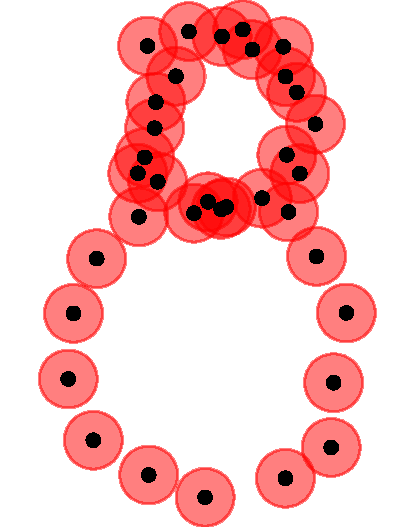
\includegraphics[width=0.4\linewidth]{figures/P8_0.4.pdf}
        \label{fig:p8_04}
    }
        \subfloat[PB up to $\epsilon=0.4$]{%
        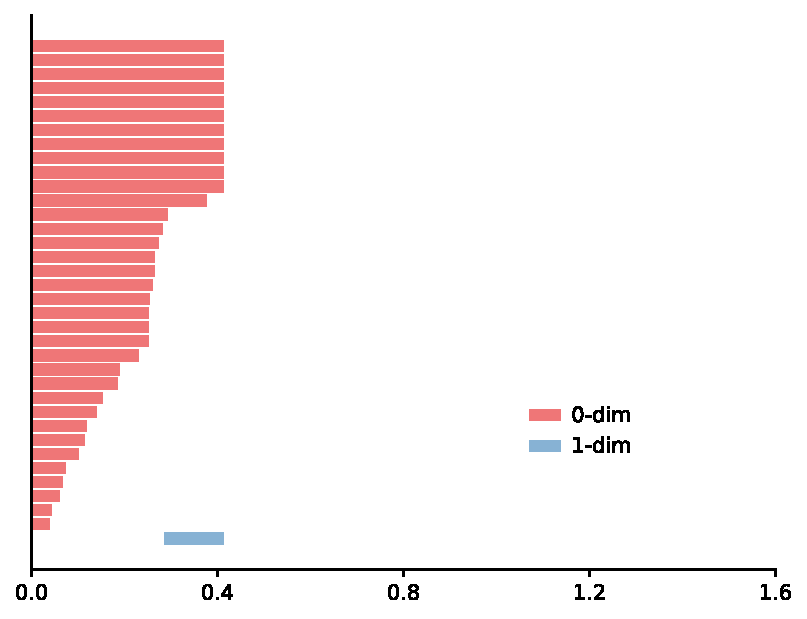
\includegraphics[width=0.6\linewidth]{figures/PBarcode_0.4.pdf}
        \label{fig:pbarcode_04}
    }
    
    \subfloat[$\epsilon=0.7$]{%
        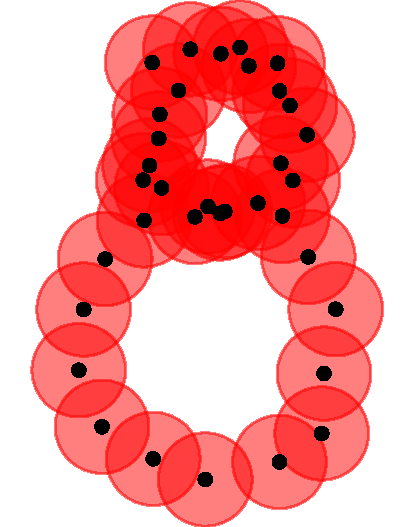
\includegraphics[width=0.4\linewidth]{figures/P8_0.7.pdf}
        \label{fig:p8_07}
    }
        \subfloat[PB up to $\epsilon=0.7$]{%
        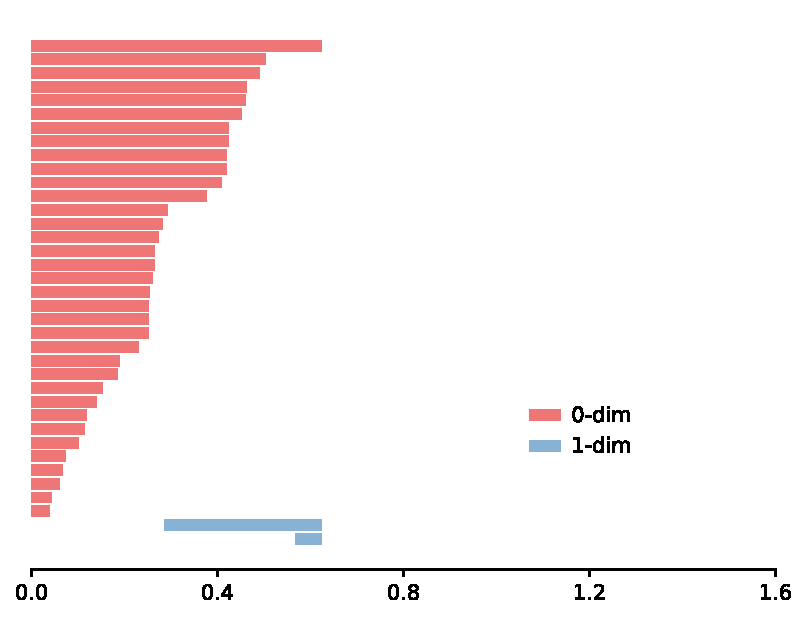
\includegraphics[width=0.6\linewidth]{figures/PBarcode_0.7.pdf}
        \label{fig:pbarcode_07}
    }
    
    \subfloat[$\epsilon=2$]{%
        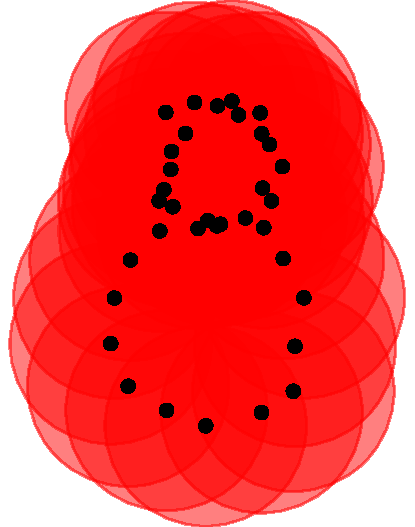
\includegraphics[width=0.4\linewidth]{figures/P8_2.pdf}
        \label{fig:p8_2e}
    }
    \subfloat[Persistence barcode]{%
        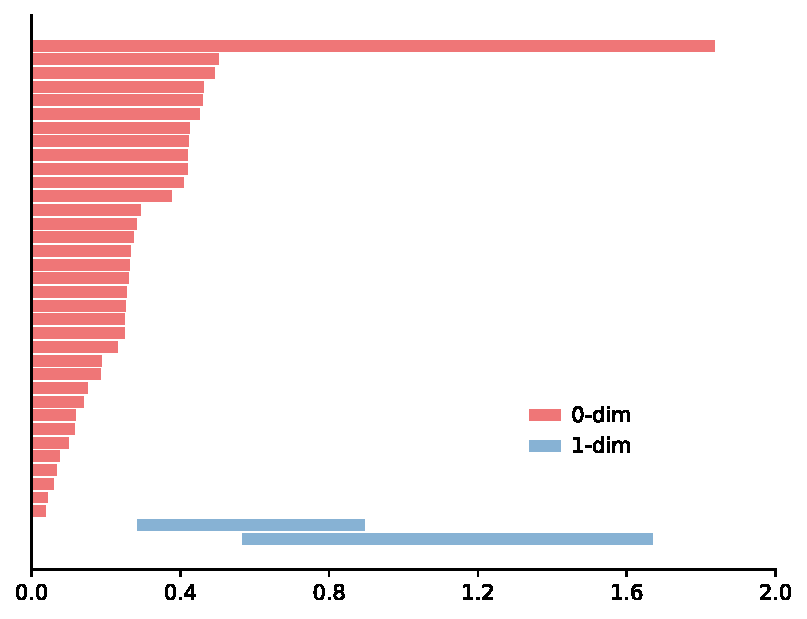
\includegraphics[width=0.6\linewidth]{figures/PBarcode_2.pdf}
        \label{fig:pbarcode_2}
    }
    \caption{\footnotesize {\bf Evolution of Persistence Barcode (PB).} In PBs shown on the right, red bars represent $\mathrm{PB}_0(\X)$, and blue bars represent $\mathrm{PB}_1(\X)$. The 8-shaped point cloud $\X$ with 35 points,  initially has 35 components, corresponding to 35 red bars. As $\epsilon$ increases, these components merge. At $\epsilon = 0.4$, only the top 11 red bars remain (b), indicating the number of components in $\mathcal{N}_{0.4}(\X)$ (a). By $\epsilon = 0.7$, the space becomes fully connected (c), and all red bars in $\mathrm{PB}_0(\X)$ terminate, except for the top $\infty$-bar (d). Regarding loops (1-holes), a small loop appears around $\epsilon = 0.3$ (a-b) and persists in $\mathcal{N}_{0.7}(\X)$ (c), while a larger loop emerges around $\epsilon = 0.6$ (d). In $\mathrm{PB}_1(\X)$ (f), two blue bars, $[0.3, 0.9)$ and $[0.6, 1.7)$, correspond to the small and large loops in the 8-shape. \label{fig:point_filtration2} }  
\vspace{-.3in}
\end{wrapfigure}



For point clouds, the number of thresholds directly determines the filtration's resolution. While thresholds are generally evenly spaced, in the presence of outliers, they can be more sparsely distributed after a certain value. Additionally, since computational cost is often a concern with point clouds, it's important to find a balance between the number of thresholds and the associated computational expense.

 

\subsection{Persistence Diagrams} \label{sec:PD}

 
After constructing the filtration $\K_1 \subset \K_2 \subset \dots \subset \K_n$ for a data type $\X$, PH systematically tracks the evolution of topological features ($k$-holes) in the filtration sequence and records this information in a \textit{persistence diagram}, which we define next. The nontrivial elements in the homology groups $\h_k(\K_i)$ for $1\leq i\leq n$ represent the $k$-dimensional topological features (or $k$-holes) appearing in the filtration sequence. Furthermore, the inclusion map $\iota: \K_i \hookrightarrow \K_{i+1}$ allows us to determine if a $k$-hole $\sigma$ in $\K_i$ persists in $\K_{i+1}$ through the induced map $\iota_*: \h_k(\K_i) \to \h_k(\K_{i+1})$.



For each $k$-hole $\sigma$, PH records its first appearance in the filtration sequence, denoted $\K_{i_0}$, and its first disappearance in a later complex, $\K_{j_0}$. We define $b_\sigma = \epsilon_{i_0}$ as the \textit{birth time} of $\sigma$ and $d_\sigma = \epsilon_{j_0}$ as the \textit{death time} of $\sigma$, where $\{\epsilon_i\}_{1}^n$ is the threshold set used for the filtration. The difference $d_\sigma - b_\sigma$ is called the \textit{lifespan} of $\sigma$. For example, if a $k$-hole $\tau$ first appears in $\K_3$ and disappears in $\K_7$, we mark the birth time as $b_\tau = \epsilon_3$ and the death time as $d_\tau = \epsilon_7$. The lifespan of $\tau$ is then $\epsilon_7 - \epsilon_3$.

 
 



 


For each nontrivial $\sigma \in \h_k(\K_i)$ for $1 \leq i \leq n$, we represent $\sigma$ with a 2-tuple $(b_\sigma, d_\sigma)$ to denote its birth and death times in the filtration. The collection of all such 2-tuples is called the \textit{persistence diagram} (PD) as depicted in Figure~\ref{fig:PD}. Note that a topological feature with the same birth and death time ($0$ lifespan) is considered a trivial topological feature, and they are represented with diagonal elements in the persistence diagrams. Therefore, the diagonal $\Delta=\{x=y\}\subset \R^2$ is always included in any persistence diagram. %Let $0 \leq k \leq D$, where $D$ is the highest dimension in the simplicial complex $\K_n$. 
Then, $k^{th}$ persistence diagram is defined as
$$\PD_k(\X)=\{(b_\sigma, d_\sigma) \mid \sigma \in \h_k(\K_i) \text{ for } b_\sigma \leq i < d_\sigma\}\cup \Delta$$

Since trivial elements $(t,t)$ in PDs can appear multiple times, we take the diagonal $\Delta$ with infinite multiplicity. Essentially, the persistence diagram is a subset of $\R^2$ ($\PD_k(\X) \subset \R^2$), where each point in $\PD_k(\X)$ is either a pair of threshold values $(\epsilon_i, \epsilon_j)$ for some $i < j$, or belongs to the diagonal (trivial element). Here, infinite multiplicity is a technical assumption, which will be important when discussing Wasserstein distance between PDs~(\Cref{sec:wasserstein}).

\begin{wrapfigure}{r}{3in}
\vspace{-.15in}
    \centering
    \subfloat[$\epsilon=2$]{%
        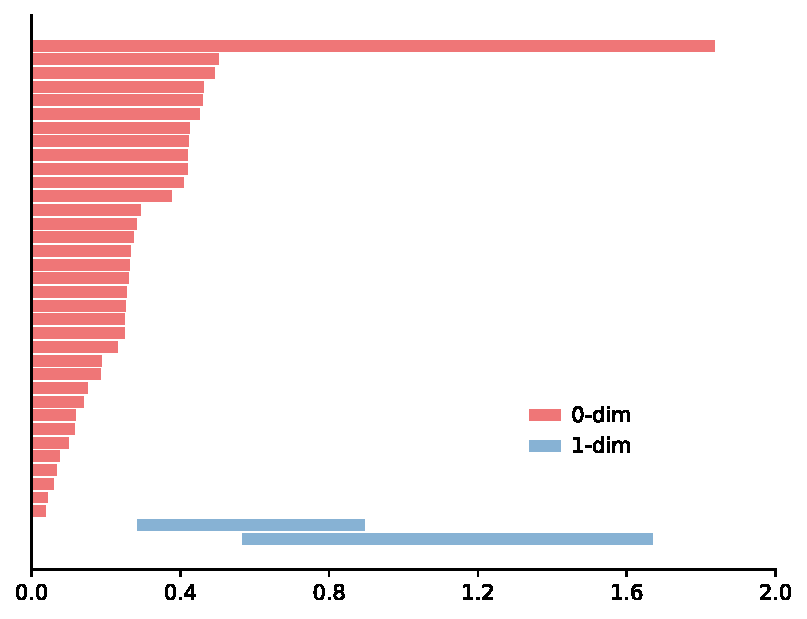
\includegraphics[width=0.5\linewidth]{figures/PBarcode_2.pdf}
        \label{fig:p8_2s}    }
    \subfloat[Persistence barcode]{%
        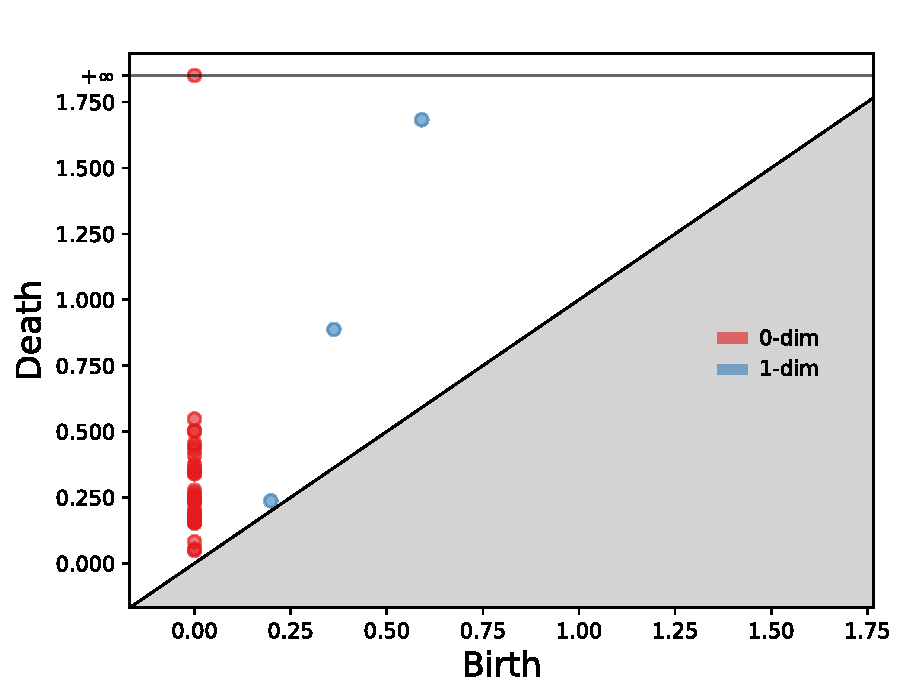
\includegraphics[width=0.5\linewidth]{figures/PDiagram.pdf}
        \label{fig:pbarcode_2b}}
       \caption{\footnotesize Persistence Barcode (left) and Persistence Diagram (right) for the 8-shaped point cloud $\X$~(\Cref{fig:point_filtration2}). Both representations convey the same information, while the PD plots each bar's birth time as its $x$-coordinate and death time as its $y$-coordinate. For example, the 35 red bars in $\mathrm{PB}_0(\X)$ that begin at 0 are represented as 35 red points along the $x=0$ line in $\PD_0(\X)$, where the $y$-coordinates correspond to the bars' death times. Similarly, the blue points at $(0.3, 0.9)$ and $(0.6, 1.7)$ represent the blue bars $[0.3, 0.9)$ and $[0.6, 1.7)$, respectively. \label{fig:PD}} 
              \vspace{-.15in}
       \end{wrapfigure}

        


There is an equivalent concept called the \textit{persistence barcode} (see Figure~\ref{fig:point_filtration2}), which uses bars (half-open intervals) $\{[b_\sigma, d_\sigma)\}$ instead of 2-tuples $\{(b_\sigma, d_\sigma)\}$. The bar notation $[b_\sigma, d_\sigma)$ represents the entire lifespan of a topological feature $\sigma$ as such an interval. In practice, persistence diagrams are more commonly used due to their practicality in applications.
 

Note that the choice between sublevel and superlevel filtration is irrelevant for the point cloud setting. In the image setting, this choice is not essential, as they essentially convey the same information due to Alexander duality~\cite{hatcher2002algebraic}; when analyzing the topological features of images, the choice of focusing on either the binary image or its complement is not crucial because the topological information of one is directly related to the topological information of the other through this duality. The Alexander duality holds only when the ambient space is quite simple, such as when the space has a structure like an $ m \times n $ rectangle, like images. However, sublevel and superlevel filtrations can yield significantly different results in the graph setting. Carriere et al.~\cite{carriere2020perslay} introduced \textit{extended persistence diagrams} to address this issue.  
This approach enables the birth and death pairs of the persistence diagram to be positioned below the diagonal ($b > d$). By doing so, it captures topological features identified through both superlevel and sublevel filtrations.

 
 
\vspace{-.1in}

 

\subsubsection{Interpretation of Persistence Diagrams}
A persistence diagram $\PD_k(\mathcal{X})$ records the $k$-dimensional topological features of the data $\mathcal{X}$ as a collection of points in $\mathbb{R}^2$. For example, $\PD_0(\mathcal{X})$ records $0$-holes (components), and $\PD_1(\mathcal{X})$ records $1$-holes (loops) appearing in the filtration sequence $\{\mathcal{K}_i\}$. Each point $q_j = (x_j, y_j)$ represents a $k$-dimensional hole $\sigma_j$. For instance, consider a threshold set $\mathcal{I} = \{\epsilon_i = i/10\}_{i=0}^{100}$ with 100 thresholds spanning the interval $[0, 10]$. Suppose we have two points, $q_1 = (0.3, 9.7)$ and $q_2 = (4.2, 4.6)$, in $\PD_2(\mathcal{X})$. These points represent $2$-holes (cavities) $\sigma_1$ and $\sigma_2$ that appear in the filtration $\mathcal{K}_0 \subset \mathcal{K}_1 \subset \dots \subset \mathcal{K}_{100}$.

For $q_1 = (0.3, 9.7)$, the cavity $\sigma_1$ first appears in $\mathcal{K}_3$ and persists until $\mathcal{K}_{97}$, indicating a long lifespan. Conversely, for $q_2 = (4.2, 4.6)$, the cavity $\sigma_2$ first appears in $\mathcal{K}_{42}$ and persists only until $\mathcal{K}_{46}$, indicating a short lifespan. This suggests that $\sigma_1$ represents an important topological feature of the data $\mathcal{X}$, while $\sigma_2$ is likely just \textit{topological noise}.

In general, features with long lifespans (where $y - x$ is large) are located \textit{far from the diagonal} and are considered significant (or "big") features. Features with short lifespans (where $y - x$ is small) are \textit{close to the diagonal} and are considered insignificant (or "small") features. This is why many vectorization techniques try to involve the lifespan information in their computation to give different emphasis to small and big features in the output.

\subsubsection{Wasserstein Distance} \label{sec:wasserstein}

After obtaining the persistence diagrams (PDs) for two datasets, $\mathbf{X}^+$ and $\mathbf{X}^-$, we can assess their topological similarities using these diagrams. One effective approach is to employ a metric in the space of PDs. If the distance between the two persistence diagrams is small, we can conclude that the two datasets exhibit similar topological characteristics; otherwise, they differ.
The most commonly used metric for this purpose is the \textit{Wasserstein distance} (also known as the \textit{matching} or \textit{earth mover distance}) of the Optimal Transport Theory (see an ICML tutorial in~\cite{bunne2023optimal}), which is defined as follows:

Let $\PD(\X^+)$ and $\PD(\X^-)$ be the persistence diagrams for the datasets $\X^+$ and $\X^-$, respectively (we omit the dimensions in PDs for simplicity). Denote $\PD(\X^+) = \{q_j^+\} \cup \Delta$ and $\PD(\X^-) = \{q_l^-\} \cup \Delta$, where $\Delta$ represents the diagonal (indicating trivial cycles) with infinite multiplicity, and $q_j^\pm = (b^\pm_j, d_j^\pm) \in \PD(\X^\pm)$ represents the birth and death times of a topological feature $\sigma_j$ in $\X^\pm$. Let $\phi: \PD(\X^+) \to \PD(\X^-)$ represent a bijection (matching). The presence of the diagonal $\Delta$ on both sides ensures the existence of these bijections even if the cardinalities $|\{q_j^+\}|$ and $|\{q_l^-\}|$ differ. This means that for optimal matching, some points in $\{q_j^+\}$ and $\{q_l^-\}$ are matched to diagonal elements whenever necessary. Then, the $x^{th}$ Wasserstein distance $\W_p$ is defined as
\[
\W_p(\PD(\X^+), \PD(\X^-)) = \min_{\phi} \left( \sum_j \|q_j^+ - \phi(q_j^+)\|_\infty^p \right)^{\frac{1}{p}}, \quad p \in \mathbb{Z}^+.
\]

Here, $\|(x_1,y_1)-(x_2,y_2)\|_\infty=\sup \{|x_1-y_1|,|x_2-y_2|\}$ is called {\em supremum norm} (or $l^\infty$-norm). When $p=\infty$, $\W_\infty$ is called the {\em bottleneck distance}. i.e.,
$\W_\infty(\PD(\X^+), \PD(\X^-)) = \max_j \{\|q_j^+ - \phi(q_j^+)\|_\infty\}$ (See \Cref{fig:wasserstein}).



\begin{wrapfigure}{r}{2.5in}
    \centering
     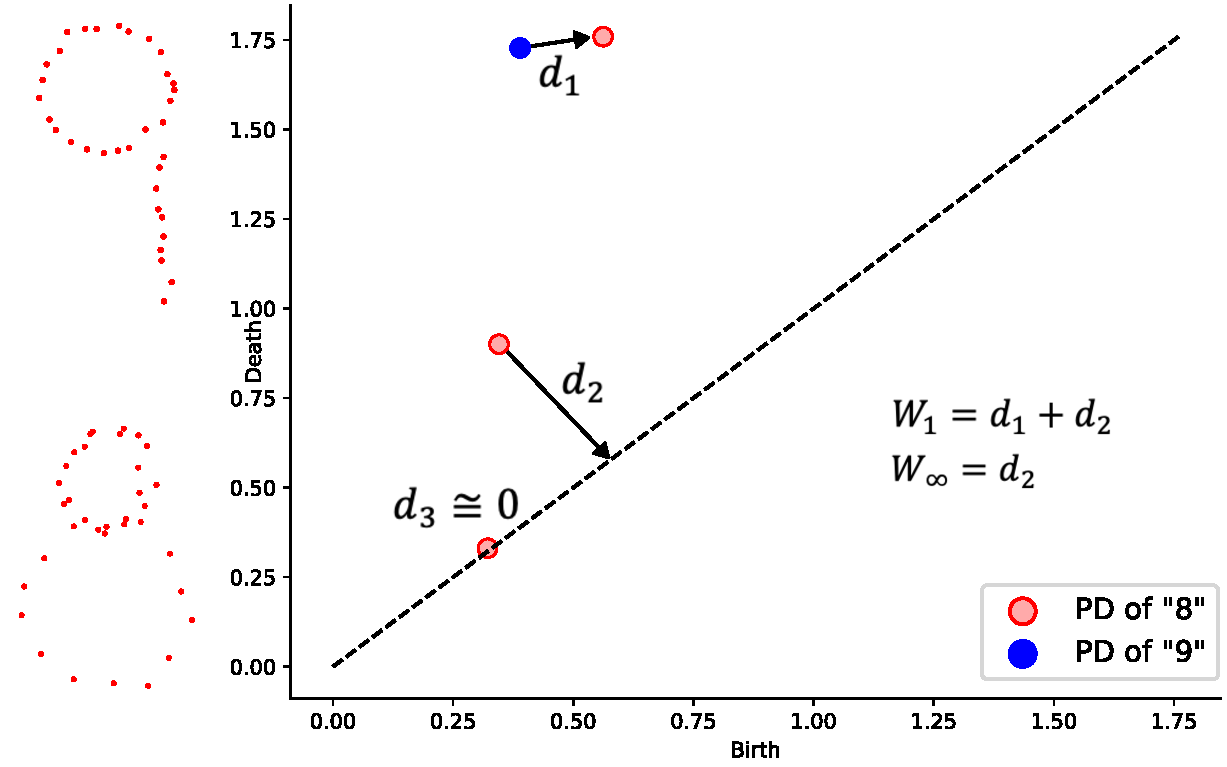
\includegraphics[width=\linewidth]{figures/pd_8_and_9.pdf}
    \caption{Wasserstein distances $\W_1$ and $\W_\infty$ (bottleneck) between $\PD_1(8)$ and $\PD_1(9)$ for the point clouds of "8" and "9" on the left.}
    \label{fig:wasserstein}
    \vspace{-.1in}
\end{wrapfigure}
In applications, the most common choices for the Wasserstein distance are $ p=1, 2, $ and $ \infty $. The bottleneck distance, unlike the $p$-Wasserstein distance, is insensitive to the number of points in $ \PD_k(\X^\pm) $ and instead focuses on the distance between the farthest points in the optimal matching. For instance, ignoring the diagonal, if $ \PD_k(\X^+) $ has 100 points and $ \PD_k(\X^-) $ has only three points, the bottleneck distance is primarily determined by finding the three closest points in $ \PD_k(\X^+) $ to those in $ \PD_k(\X^-) $ and taking the maximum of these distances. Conversely, when using $ p=1 $ or $ p=2 $, the quantity of points in $ \PD_k(\X^\pm) $ becomes significant as all points contribute to the distances, even if only slightly. Therefore, if there are only a few points in $ \{\PD_k(\X_j)\} $ and the focus is on the distances of the most critical features, the bottleneck distance is preferable. However, if there are many points in $ \{\PD_k(\X_j)\} $ and the primary topological patterns arise from the quantity and location of smaller features, then choosing $ p=1 $ (or $ p=2 $) for the Wasserstein distance would be more suitable. 
 

There are several ways to utilize the Wasserstein distance in applications. One common approach is to bypass the vectorization step, which requires some choices, and directly compare persistence diagrams. For instance, to determine if two datasets have similar shapes or structures, one can compute the persistence diagrams for both datasets and then calculate the Wasserstein distance between these diagrams. A smaller distance indicates more similar shapes. Another application lies in unsupervised learning, where datasets are clustered based on their topological similarity using persistence diagrams, utilizing the Wasserstein distance to measure distances between them.


\subsection{Integrating PDs to ML tasks 1: Vectorizations} \label{sec:vectorization}

To effectively use persistence diagrams (PDs) in ML applications, it is crucial to convert them into numerical or vector formats, allowing for the seamless integration of TDA outputs into standard ML workflows. Although PDs capture the birth and death of topological features within data, their variable size and structure make them challenging to handle directly. For example, in a binary graph classification task with 1000 graphs (400 in Class A and 600 in Class B), PDs might visually highlight differences between the classes. However, applying traditional statistical tools to PDs, which are subsets of $\R^2$, is problematic; for instance, it is not possible to compute averages or confidence intervals for each class. Moreover, directly inputting PDs into ML models is impractical because their variable point count conflicts with the fixed-size input required by most ML algorithms.

Vectorization addresses this by making PDs compatible with traditional ML and statistical techniques. Below, we outline the most common vectorization methods used in practice. For a comprehensive review, refer to~\cite{ali2023survey}.


 

In the following, for a fixed dataset $\mathcal{X}$, a threshold set $\{\epsilon_i\}_{i=1}^n$, and an induced filtration $\{\mathcal{K}_i\}_{i=1}^n$, we will introduce several vectorization methods. It is important to note that all these vectorization methods are applicable to any type of data since they simply transform a given PD into vectors. However, the effectiveness and common usage of certain vectorization methods can vary depending on the data type and the density or sparsity of the PDs. Although we present various vectorization methods and their configurations here, \textit{those who prefer to avoid the intricacies of vectorization selection and hyperparameter tuning can opt for automated approaches, as detailed in~\Cref{sec:vecNN}}.
 

\paragraph*{Function vs. Vector Format.} In the following, we introduce several vectorization methods. For each method, we will describe how to convert a given PD into a \textit{vector} or a \textit{function} depending on the setting. Depending on the context, one of these formats might be preferable (visualization, ML input, etc.), however, both formats can be easily converted to each other. For example, if we have a function $f:[\epsilon_1,\epsilon_n]\to\mathbb{R}$ defined over an interval, we can convert $f$ into an $N$-dimensional vector by sampling the values at $f(t_j)$ where $t_j = \epsilon_1 + \frac{j}{N}(\epsilon_n - \epsilon_1)$ and $j$ ranges from 1 to $N$. For each point $t_j$, we calculate $f(t_j)$. The vector $\mathbf{v}_f$ is then  $\mathbf{v}_f=[f(t_1), f(t_2), \dots, f(t_N)]$. Conversely, for a given $N$-dimensional vector $\mathbf{v}=[v_1 \ v_2 \ \dots v_N]$, we can convert it to a function via a step function or linear spline interpolation, e.g., $g_\mathbf{v}:[\epsilon_1,\epsilon_n]\to\mathbb{R}$ such that $g_\mathbf{v}(t_j)=v_j$ for $t_j=\epsilon_1+\frac{j}{N}(\epsilon_n-\epsilon_1)$. Then, for any point $s\in[t_j,t_{j+1}]$, we define the linear extension $g(s)=g(t_j)+\frac{g(t_{j+1})-g(t_j)}{t_{j+1}-t_j}(s-t_j)$. Hence, any of the following vectorizations can be taken as a function or vector depending on the need.


\paragraph*{Topological Dimensions and Final Topological Vector.} In each vectorization method, we convert a persistence diagram $\PD_k(\X)$ into a vector (or array) $\mathbf{v}_k$ where $k$ represents a topological dimension of $k$-holes. In particular, each persistence diagram produces a different vector. The user needs to decide which topological dimensions to be used in the method. After getting an $N$-dimensional vector for each dimension, a common method is to concatenate them to obtain the final topological vector. Hence, if we use $m$ different topological dimensions, we have $(m\cdot N)$-dimensional final vector $\mathbf{v}(\X)=\mathbf{v}_0\mathbin\Vert \mathbf{v}_1\mathbin\Vert \dots\mathbin\Vert \mathbf{v}_{m-1}$. In most applications, the common dimensions used are $k=0$ and $k=1$, and hence the final topological vector is $2N$-dimensional, i.e., $\mathbf{v}(\X)=\mathbf{v}_0\mathbin\Vert \mathbf{v}_1$.


\paragraph*{Betti vectors} One of the most straightforward and interpretable vectorization methods in TDA is the {\em Betti function}. The $k^{\text{th}}$ Betti number of a topological space $\K$ essentially counts the total number of $k$-dimensional holes in $\K$. More formally, it is defined as $\beta_k(\K) = \text{rank}(H_k(\K))$, which is the rank of the $k^{\text{th}}$ homology group of $\K$. For example, $\beta_0(\K)$ represents the number of connected components in $\K$, while $\beta_1(\K)$ indicates the number of $1$-dimensional holes.



\begin{wrapfigure}{r}{0.4\linewidth}
\vspace{-.1in}
\centering
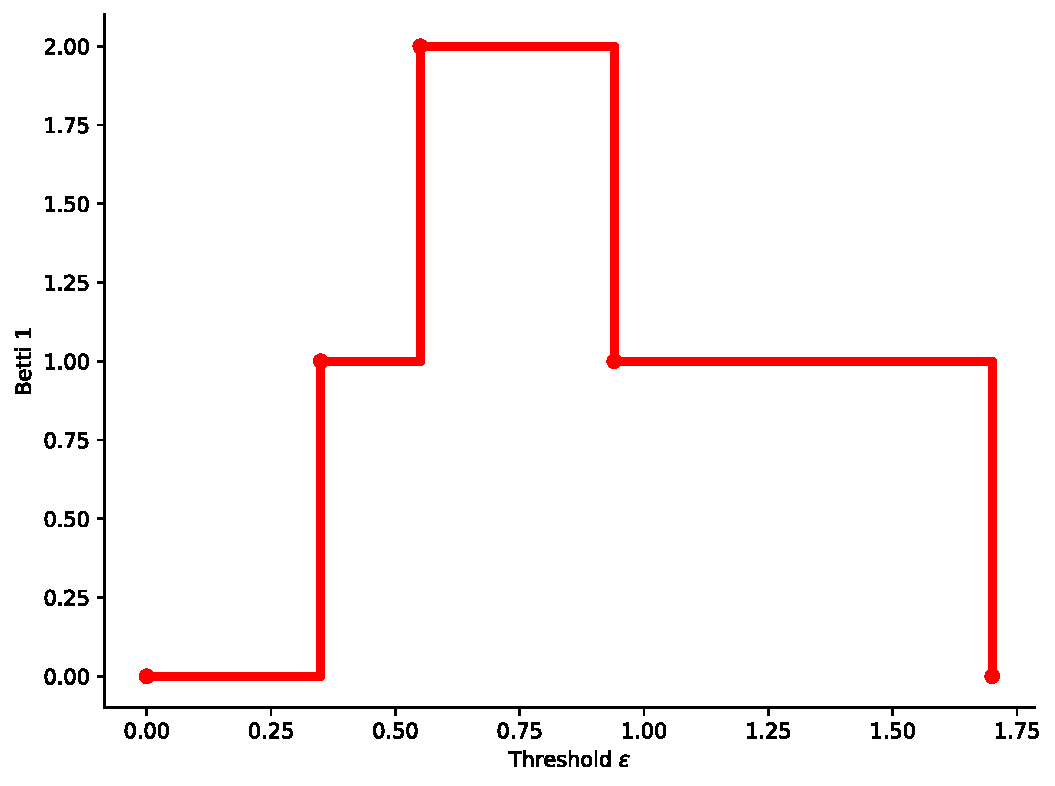
\includegraphics[width= 0.98\linewidth]{figures/bettifunction}
\caption{\footnotesize \textbf{Betti Function.} The step function represents the first Betti number ($\beta_1$) over the figure-eight-shaped point cloud of Figure~\ref{fig:graph-filtration} as a function of the threshold $\epsilon$. The function shows the number of 1-dimensional holes (loops) in the point cloud. Initially, there are no loops ($\beta_1 = 0$), then a single loop appears at $\epsilon = 0.35$ and persists until $\epsilon = 0.94$, during which another loop appears at $\epsilon = 0.55$ and vanishes at $\epsilon = 0.94$. The final loop disappears at $\epsilon = 1.70$, returning $\beta_1$ to 0. 
 \label{fig:betti_function}} 
 \vspace{-.2in}
\end{wrapfigure}
For given filtration $\{\K_i\}_1^n$, we define $k^{th}$  Betti vector $\vec{\beta}_k(\X)= [ \beta_k(\K_1) \ \beta_k(\K_2) \dots \beta_k(\K_n)]$. Therefore, for each topological dimension $k$, we obtain a Betti vector of the size of a number of thresholds. For example, $k=0,1$ with $n=50$ results in $50$-dimensional vector for each dimension. In ML applications, typically, these vectors are concatenated to create a $100$-dimensional topological vector as output.





\begin{example} \label{ex:betti} Consider the point cloud $\X$ in~\Cref{fig:point_filtration2}. We define a filtration using five threshold values $\wh{\epsilon} = [0, 0.25, 0.75, 1.5, 1.75]$, where $\K_i = \N_{\e_i}(\X)$. The Betti-0 vector $\vec{\beta}_0(\X) = [35, 20, 1, 1, 1]$ is obtained, with $\beta_0(\X) = 35$, $\beta_0(\N_{0.25}(\X)) = 20$, and $\beta_0(\N_\epsilon(\X)) = 1$ for $\epsilon \geq 0.7$. This indicates that $\N_{0.25}(\X)$ consists of 20 connected components. The Betti-0 vector can be easily determined from the persistence barcode $\mathrm{PB}_0(\X)$~(\Cref{fig:pbarcode_2}) by counting the number of red bars intersected by a vertical line $x=\e_i$, representing the number of persistent topological features at the threshold $\e_i$. Thus, with 5 thresholds, we obtain a 5-dimensional vector, $\vec{\beta}_0(\X)$.




Similarly, we can determine the corresponding Betti-1 vector by examining the blue bars in the persistence barcode~(\Cref{fig:pbarcode_2}). We observe no blue bar at $x = 0$, $0.25$, and $1.75$. Furthermore, there are two blue bars at $x = 0.75$ and one blue bar at $x = 1.5$. Therefore, the Betti-1 vector is $\vec{\beta}_1(\X) = [0, 0, 2, 1, 0]$. This indicates that there are no 1-dimensional holes (1-holes) in $\X = \N_0(\X)$, $\N_{0.25}(\X)$, or $\N_{1.75}(\X)$, while $\N_{0.75}(\X)$ contains two 1-holes and $\N_{1.5}(\X)$ contains one. It is also common to use Betti vectors as Betti functions via step functions~(See~\Cref{fig:betti_function}).
Similarly, using 21 equally spaced thresholds $\wh{\e} = \{0, 0.1, 0.2, \dots, 2\}$ would yield 21-dimensional vectors $\vec{\beta_0}$ and $\vec{\beta_1}$.
\end{example}

We note that Betti vectors do not require the computation of persistence diagrams. Therefore, there are computationally more effective ways to produce Betti vectors~\cite{hayakawa2022quantum,ameneyro2024quantum}. Another favorable aspect of Betti vectors is their \textbf{ease of interpretation}. Simply put, $\beta_k(\epsilon_i)$ is equal to the number of $k$-dimensional topological features in $\mathcal{K}_i$.



 \begin{wrapfigure}{r}{2in}
\vspace{-.15in}
\centering
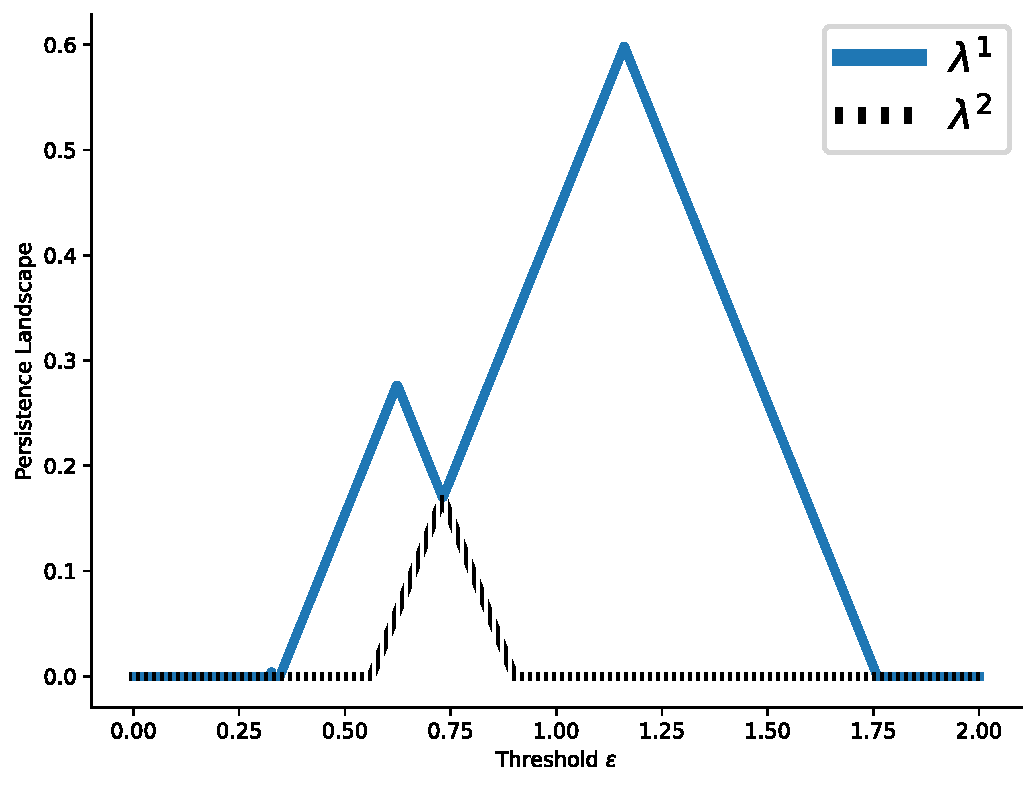
\includegraphics[width= 0.98\linewidth]{figures/landscape.pdf}
\caption{\textbf{Persistence Landscape (PL).} The plot shows the PL for $\PD_1(\X)$ for the 8-shaped point cloud filtration in~\Cref{ex:betti}. In the plot, the blue function corresponds to $\lambda^1$, and the orange function to $\lambda^2$. \label{fig:landscape}}
\vspace{-.15in}
\end{wrapfigure}

\paragraph*{Persistence Landscapes} Persistence Landscapes are one of the first vectorization methods in TDA, introduced by P. Bubenik, directly utilizing the lifespan information~\cite{bubenik2015statistical}. In particular, in this vectorization, the points away from the diagonal (large features) are easily distinguished and promoted. For a given persistence diagram $\PD_k(\X)=\{(b_i,d_i)\}$, we first define generating functions $\Lambda_i$ for each $(b_i,d_i)\in \PD_k(\G)$, i.e., $\Lambda_i:[b_i,d_i]\to\R$ is a piecewise linear function obtained by two line segments starting from $(b_i,0)$ and $(d_i,0)$ connecting to the same point $(\frac{b_i+d_i}{2},\frac{b_i-d_i}{2})$. Then, we define several piecewise-linear functions $\{\lambda^m\}$ in the following way. For each $t\in[\epsilon_1,\epsilon_n]$, we check all generating functions $\{\Lambda_i(t)\}$, and we mark $m^{th}$ largest value. In particular, $m^{th}$ \textit{Persistence Landscape} function $\lambda^m(\X):[\epsilon_1,\epsilon_n]\to\R$ for $t\in [\epsilon_1,\epsilon_n]$ is defined as $\lambda^m(\X)(t)=m^{th}\ \max_i\{\Lambda_i(t)\}$ (See~\Cref{fig:landscape}). Note that the first and second persistence landscapes are the most commonly used vectors, and they are used with concatenation in the applications. 
 


  \begin{wrapfigure}{r}{2.5in}
 %\vspace{-.15in}
\centering
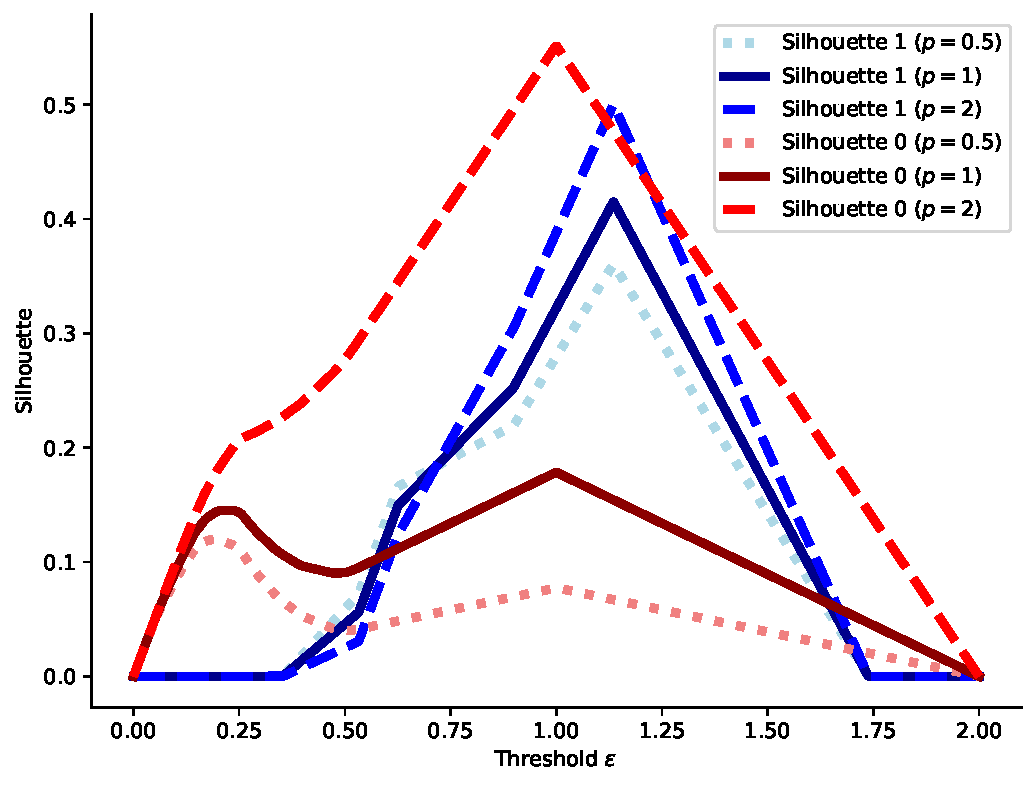
\includegraphics[width=\linewidth]{figures/silhouette.pdf}
\caption{\footnotesize \textbf{Silhouette Functions.} The plot shows the silhouette functions with tuning parameters $p=0.5,1,2$ $\PD_1(\X)$ for the 8-shaped point cloud filtration given in~\Cref{ex:betti}. \label{fig:silhouette}}
 
\vspace{-.15in}
\end{wrapfigure}

\paragraph*{Silhouettes} While persistence landscapes are among the first vectorizations to effectively utilize lifespan information, the need to consider $m$ different maxima makes it difficult to use in ML applications.
In \cite{chazal2014stochastic}, Chazal et al. proposed a practical modification called the {\em Silhouette} for persistence landscapes. This modification introduces a tuning parameter $p$ to better utilize the lifespans of topological features. For a persistence diagram $\PD_k(\X)=\{(b_i,d_i)\}_{i=1}^N$, let $\Lambda_i$ be the generating function for $(b_i,d_i)$ as defined in the persistence landscapes. The \textit{Silhouette} function $\psi$ is defined as: $\Psi_k(\X)=\dfrac{\sum_{i=1}^N w_i\Lambda_i(t)}{\sum_{i=1}^m w_i}, \ t\in[\epsilon_1,\epsilon_n],$
where the weight $w_i$ is usually chosen as the lifespan $(d_i-b_i)^p$. Thus, the $p$-silhouette function $\psi^p_k(\X):[\epsilon_1,\epsilon_n]\to \R$ is defined as: 

\hspace{2cm} $\Psi^p_k(\X)=\dfrac{\sum_{i=1}^N (d_i-b_i)^p\Lambda_i(t)}{\sum_{i=1}^N (d_i-b_i)^p}$

\vspace{.1cm}

The tuning parameter $p$ is crucial as it adjusts the silhouette function's emphasis on topological features with varying lifespans. When $p<1$, shorter lifespans $(d_i-b_i)$ are given more weight, emphasizing smaller features. Conversely, shorter lifespans are down-weighted when $p>1$, highlighting larger features. Common choices for $p$ are $\frac{1}{2}$, 1, and 2 (See~\Cref{fig:silhouette}). If the persistence diagram has a few points and the goal is to emphasize significant features, $p=2$ would be a good choice. If there are many points and the key information comes from smaller features, $p=\frac{1}{2}$ is considered more suitable. Similarly, Silhouette functions $\psi^p_k(\X)$ can be converted to vectors for each dimension $k$, and concatenation of these vectors can be used in the application as the topological vector of the dataset.



 \begin{wrapfigure}{r}{2.5in}
 \vspace{-.15in}
\centering
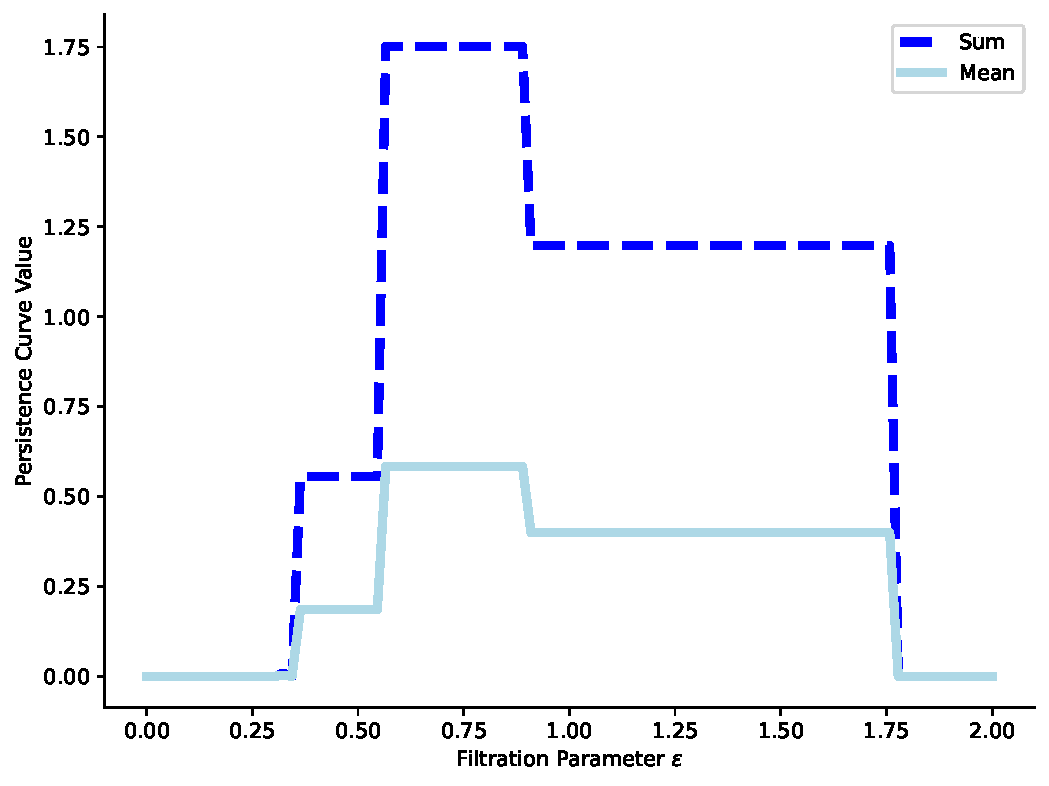
\includegraphics[width= 0.98\linewidth]{figures/per_curve.pdf}
\caption{\footnotesize \textbf{Persistence Curves.} The plot shows the persistence curves for $\PD_1(\X)$ for the 8-shaped point cloud filtration in~\Cref{ex:betti} by using two different summary statistics: sum and mean. The dashed line represents the persistence curve using the sum of lifespans, which emphasizes the cumulative contribution of all loops. The solid line represents the persistence curve using the mean of lifespans, which highlights the average significance of the loops. This visualization illustrates how different summary statistics influence the interpretation of topological features in the data.}
\label{fig:persistence_curves}
 \vspace{-.15in}
\end{wrapfigure}
\paragraph*{Persistence Curves} The Persistence Curve (PC) framework, introduced by Chung et al.~\cite{chung2019persistence}, offers a structured approach to the vectorization process. The core idea revolves around utilizing a generating function $\psi$, a summary statistic $T$, and a filtration parameter $\epsilon$. From these elements, a PC is defined as: 

$PC(\D, \psi, T )(t) = T ([\psi(\D; b, d, \epsilon) \mid (b, d) \in \D_\epsilon ]), \epsilon \in \R.$ 

Here, $\D_\epsilon$ represents the points within the persistence diagram $\D$ that fall inside a region $\Delta_\epsilon$ varying with the filtration value $\epsilon$.  
The function $\psi$ takes as input a point from the persistence diagram $\D$,  and the filtration parameter, $\epsilon$ and outputs a real number.  This function can be chosen to prioritize certain points in the PD or to emphasize specific features. Finally, the statistic $T$  acts upon a multiset of values, aggregating them into a single real number.  Common examples include sum, mean, or max.  

 
PCs provide a general and unifying framework for vectorization methods.
By selecting different combinations of $\psi$ and $T$, one can generate various functional summaries of the PD, each potentially highlighting different aspects of the data. Many established vectorizations of PDs can be represented within the PC framework, e.g., Betti curves, persistence landscapes, silhouettes, and entropy curves. See~\cite{chung2019persistence} for more details.



 

\begin{wrapfigure}{r}{3in}
\vspace{-.2in}
    \centering
    \subfloat{%
        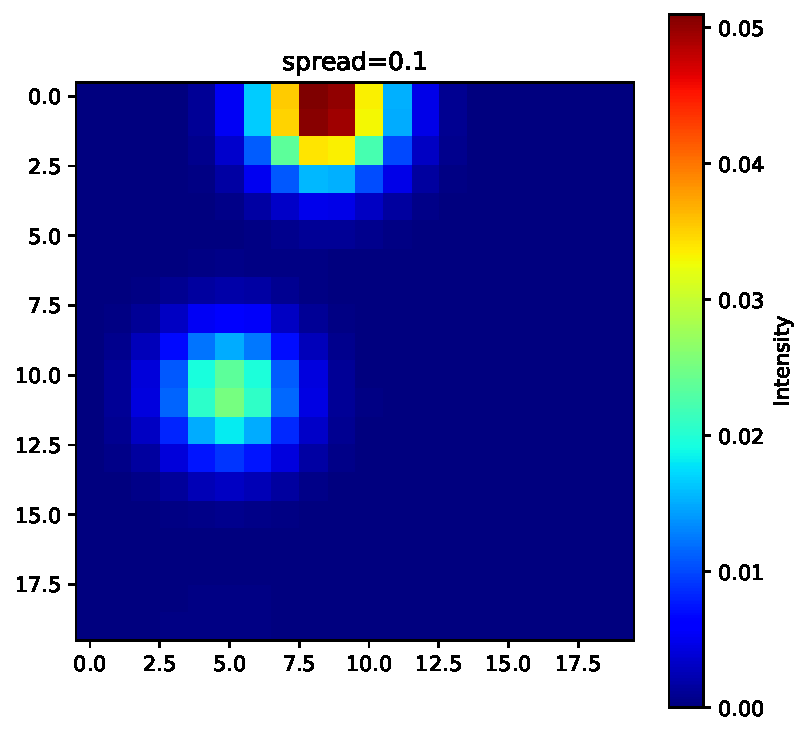
\includegraphics[width=0.32\linewidth]{figures/per_image_0.1.pdf}
        \label{fig:p8_04b}}
    \subfloat{%
        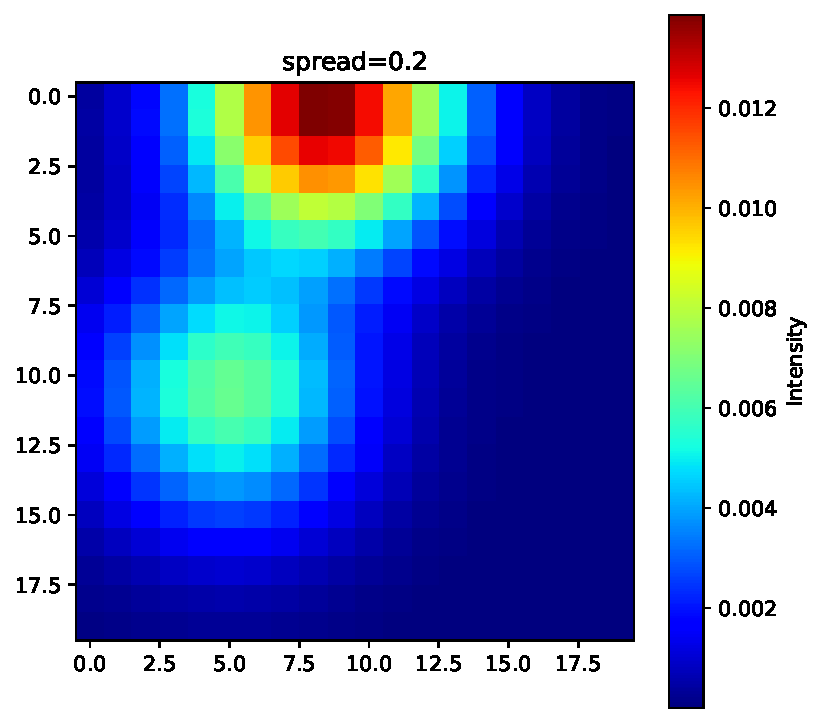
\includegraphics[width=0.33\linewidth]{figures/per_image_0.2.pdf}
        \label{fig:p8_07b}}
    \subfloat{%
        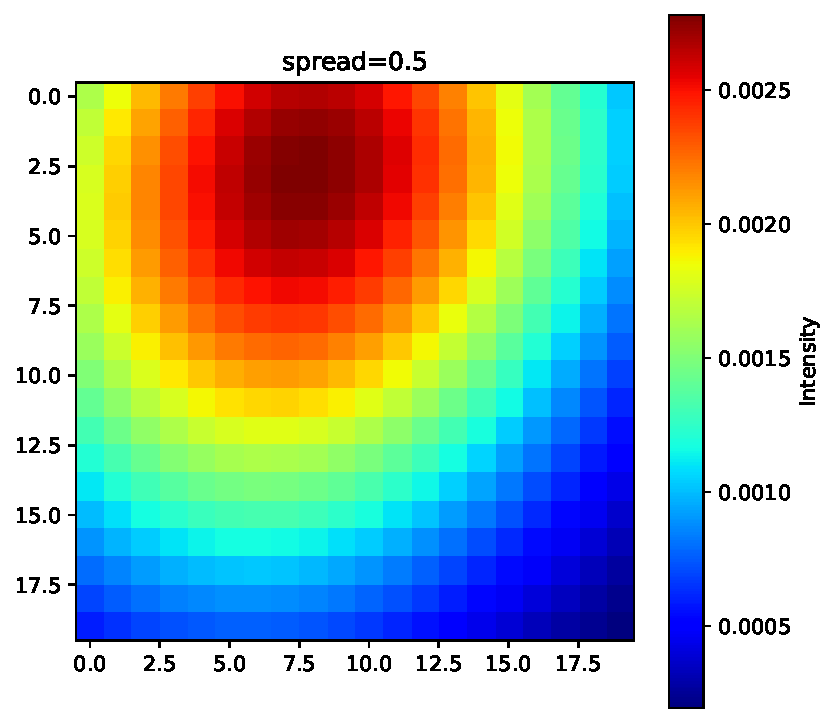
\includegraphics[width=0.34\linewidth]{figures/per_image_0.5.pdf}
        \label{fig:p8_2b}}
    \caption{\footnotesize {\bf Persistence images (PI).} PIs are vectorization with 2D (matrix) output. Here, we give examples of PIs for $\PD_1(\X)$ ($8$-shaped point cloud in \Cref{ex:betti}) with different spread values. The spread parameter $\sigma$ controls the standard deviation of the Gaussian functions used to smooth the persistence points in the persistence diagram. As illustrated in the figures, as $\sigma$ increases, the generating Gaussian functions are even more spread out, producing a flatter persistence image.    \label{fig:persistence_image}}
        
        \vspace{-.1in}
\end{wrapfigure}

\paragraph*{Persistence Images} Our next vectorization is Persistence Images, introduced by Adams et al.~\cite{adams2017persistence}. Unlike most vectorizations, Persistence Images, as the name suggests, produce $2D$-arrays (tensors). The idea is to capture the location of the points in the PDs with a multivariable function by using the $2D$ Gaussian functions centered at these points. For $PD(\G)=\{(b_i,d_i)\}$, let $\phi_i$ represent a $2D$-Gaussian centered at the point $(b_i,d_i)\in \R^2$. Then, one defines a multivariable function, \textit{Persistence Surface}, $\wt{\mu}=\sum_iw_i\phi_i$ where $w_i$ is the weight, mostly a function of the life span $d_i-b_i$. To represent this multivariable function as a $2D$-vector, one defines a $k\times l$ grid (resolution size) on the domain of $\wt{\mu}$, i.e., threshold domain of $PD(\G)$. Then, one obtains the \textit{Persistence Image}, a $2D$-vector (matrix) $\vec{\mu}=[\mu_{rs}]$  of size $k\times l$ such that 
$$\mu_{rs}=\int_{\Delta_{rs}}\wt{\mu}(x,y)\,dxdy \quad \text{where } \Delta_{rs}= \text{ pixel with index }rs \text{ in the } k\times l \text{ grid.}$$


Note that the resolution size $k\times l$ is independent of the number of thresholds used in the filtering; the choice of $k$ and $l$ is completely up to the user. There are two other important tuning parameters for persistence images, namely the weight $w_i$ and the variance $\sigma$ (the width of the Gaussian functions). Like Silhouettes, one can choose $w_i=(d_i-b_i)^p$ to emphasize large or small features in the PD. Similarly, the width parameter $\sigma$ determines the sharpness of Gaussian, where smaller $\sigma$ would make the Gaussian functions more like Dirac $\delta$-function, and larger $\sigma$ would make the Gaussians flat. Depending on the context, $\sigma$ can be chosen a constant (e.g. $\sigma=0.1$) or depending on the point $(b_i,d_i)$, e.g., $\sigma_i=k(d_i-b_i)$ for some constant $k>0$.



\paragraph*{Kernel Methods} \label{sec:kernel} Kernel methods provide an alternative to traditional direct vectorization techniques used to transform PDs into formats suitable for ML algorithms. In ML, these methods utilize a mathematical function known as a \textit{kernel} to analyze data and discern patterns. Unlike earlier approaches that directly represent PDs using vectors or functions, kernel methods compute a \textit{similarity score} as an inner product between pairs of PDs in a high-dimensional space without explicitly mapping the data. This approach is advantageous because it adapts well to ML techniques like support vector machines (SVMs) and kernel principal component analysis (KPCA). Therefore, kernel methods are well-suited for tasks such as classification, regression, and principal component analysis.

One common such method is the persistence weighted Gaussian kernel (PWGK)~\cite{kusano2016persistence}. It enhances the Gaussian kernel by incorporating weights based on the significance of topological features. This approach amplifies the influence of important features while reducing noise (i.e., short-lived holes) impact. For instance, it assigns weights to points $p=(b,d)\in\PD(\X)$ proportional to their lifespans $w(p)=(d-b)$. In particular, PWGK is defined as
\[ 
\mathbf{K}(\PD(\X^+), \PD(\X^-)) = \sum_{p \in \PD(\X^+)} \sum_{q \in \PD(\X^-)} w(p) w(q) k(p, q)
\]

where $k(p, q) = \exp\left(-\frac{\|p - q\|^2}{2\sigma^2}\right)$ denotes the Gaussian kernel function.

Another significant approach is the sliced Wasserstein kernel (SWK)~\cite{carriere2017sliced}, which computes the Wasserstein distance between PDs and integrates it into a kernel framework. This method employs Optimal Transport Theory to establish a meaningful metric for comparing PDs. Although kernel methods can yield better results in some settings, they can be computationally intensive and impractical for large datasets due to the high computational costs associated with computing the kernel matrix. In particular, computing kernels takes quadratic time in the number of diagrams, while vectorizing PDs takes only linear time.



\subsubsection{Stability} In most applications, the stability of vectorization is vital for statistical and inferential tasks. Essentially, stability means that a small change in the persistence diagram (PD) should not lead to a significant change in its vectorization. In particular, if two PDs, $\PD_k(\X^+)$ and $\PD_k(\X^-)$, are close, their corresponding vectorizations, $\vec{\beta}_k(\X^+)$ and $\vec{\beta}_k(\X^-)$, should also be close. This ensures that the vectorization process preserves the structural properties of the data. Therefore, when two persistence diagrams $\PD_k(\X^\pm)$ are similar, it implies that the datasets $\X^+$ and $\X^-$ share similar shape characteristics. If these datasets are intuitively expected to belong to the same class, their vectorizations $\vec{\beta}_k(\X^\pm)$ should likewise remain close.

To formalize this concept, we need to define what constitutes a "small/big change" or what it means for PDs to be close. This requires a distance (metric) in the space of PDs, with the most common being the \textit{Wasserstein distance} (or matching distance) as defined in \Cref{sec:wasserstein}. Similarly, we need a metric for the space of vectorizations, such as the Euclidean distance $\|\vec{\beta}(\X^+) -\vec{\beta}(\X^-)\|$ for $\vec{\beta} \in \R^N$. Thus, for a given vectorization $\vec{\beta}$, we call it stable (with respect to the Wasserstein-$p$ metric) if it satisfies the stability equation
\[ \|\vec{\beta}_k(\X^+) -\vec{\beta}_k(\X^-)\|\leq C \cdot \W_p(\PD_k(\X^+), \PD_k(\X^-)) \]
This ensures that if $\W_p(\PD_k(\X^+), \PD_k(\X^-))$ (the distance between PDs) is small, then the distance $\|\vec{\beta}_k(\X^+) -\vec{\beta}_k(\X^-)\|$ between the corresponding vectorizations will also be small.
Among the methods described earlier, persistence landscapes, silhouettes, persistence images, and most kernel methods are stable vectorizations, while Betti functions are generally unstable.


\subsubsection{Choice of Vectorization and Hyperparameters}  
The choice of vectorization method should align with the characteristics of your data and the problem at hand. If your data contains a few prominent topological features that are crucial to the task, Silhouettes with $p \geq 2$ or Persistence Images may be the most suitable options. These methods are also effective when dealing with noisy data, allowing you to filter out less significant features. Conversely, if your data generates a high number of small features, where the task hinges on their location and density—in other words, when the noise itself carries important information—Betti curves, Persistence curves, Silhouettes with $p\leq 0.5$ and kernel methods are likely to yield strong performance. On the other hand, for point cloud data, Turkes et al.~\cite{turkes2022effectiveness} provide valuable insights on how to effectively utilize PH for shape recognition. Lastly, if interpretability is a priority, Betti Curves stands out as the most interpretable vectorization method. Note that most vectorizations are computationally efficient and require minimal time compared to the computation of PDs.
%Furthermore, if the computational cost is a concern, Otter et al.~\cite{otter2017roadmap} provide a guideline for the computational costs of these vectorizations. 


\paragraph*{Hyperparameters: } Each vectorization method comes with its own set of hyperparameters that need to be carefully tuned to maximize performance. In all of them, the choice of \textit{thresholds} is one of the key hyperparameters we discussed in~\Cref{sec:threshold}.

In addition to thresholds, many vectorization methods have \textit{tuning parameters} that are used to adjust sensitivity to topological noise. Typically, topological features with short lifespans (i.e., those close to the diagonal in PDs) are regarded as noise. These features, represented as pairs \(\{(b,d)\}\) with short lifespans \((d-b)\), are generally easy to detect, leading to many tuning parameters being tied to the lifespan.
For example, in persistence landscapes, the number of landscapes (\(m\)) specifies how many maxima are included in the representation. A higher number of landscapes provides a richer depiction of topological features but increases computational complexity. The first few landscapes (e.g., \(1^{st}\) and \(2^{nd}\) landscapes) emphasize features with the largest lifespans.
In silhouettes, the tuning parameter \(p\) in the weight function \(w_i = (d_i - b_i)^p\) determines the emphasis of the vectorization. A higher \(p\) (e.g., \(p \geq 2\)) de-emphasizes features with short lifespans, while a smaller \(p\) (e.g., \(p \leq 0.5\)) increases the importance of topological noise.

For persistence images, the spread (\(\sigma\)) controls the width of the Gaussian kernels applied to each persistence point. A smaller spread results in sharper, more localized features, whereas a larger spread yields smoother images. The resolution parameter sets the number of pixels in the persistence image, thus determining the output dimension of the vectorization. Higher resolution captures finer detail but at a higher computational cost. Similar to silhouettes, a weight function (e.g., linear) can be applied to weigh the contribution of each persistence point based on its significance, such as its lifespan.


\subsection{Integrating PDs to ML tasks 2: Using Neural Networks} \label{sec:vecNN}

While vectorization choices provide greater control over the model and data analysis, there are automated methods to avoid dealing with vectorization choices or hyperparameter tuning. These methods optimize the selection for downstream tasks by either finding the best vectorization within a large vectorization space or working directly with persistence diagrams as point clouds, allowing neural networks to handle the data.

\subsubsection{Vectorization with NN: Perslay} \label{sec:perslay} PersLay, introduced by Carrière et al.~\cite{carriere2020perslay}, is an automated vectorization framework for persistence diagrams, which decides the best vectorization method for the downstream task. The method leverages a neural network architecture that processes PDs via a specialized layer called the PersLay layer. This layer incorporates a variety of vectorization strategies, providing a unified and flexible approach to extracting topological features.

The PersLay layer is composed of several key components: 
\begin{itemize}
    \item {\em Weighting Functions:} These assign importance to points in the persistence diagram. Common choices include exponential weighting and Gaussian weighting, which can be learned during training.
\item {\em Transformation Functions:} These functions, such as linear transformations or learned neural networks, apply to the coordinates of the persistence points to encode meaningful geometric and topological information.
\item {\em Symmetric Functions:} After transformation, symmetric functions like sum, mean, or max aggregate the transformed points into a fixed-size vector, ensuring permutation invariance.
\end{itemize}

With this architecture, PersLay covers a wide range of known vectorization methods within its framework, i.e., Persistence Landscapes, Persistence Images, Silhouettes, Betti Curves, Entropy Functions and other Persistence Curves~\cite{chung2019persistence}. By incorporating various vectorization techniques, PersLay can adapt to diverse data types and topological features, making it a robust and versatile tool for integrating PH into ML workflows. For an alternative method involving slightly different generating functions for learnable vectorizations, see~\cite{hofer2019learning} by Hofer et al.
 
 

\subsubsection{PD Learning with NN: PointNet} \label{sec:pointnet} An alternative automated method to leverage PDs in ML tasks without hyperparameter tuning is to directly utilize PointNet~\cite{qi2017pointnet} or similar neural network architectures to process and analyze point cloud data, e.g., DeepSets~\cite{zaheer2017deep}, PointMLP~\cite{ma2022rethinking}. Unlike conventional techniques that transform point clouds into regular grids or structured formats, these networks treat PDs as sets of points in $\mathbb{R}^2$. Perslay and PointNet offer fundamentally different strategies for incorporating PDs into ML models without requiring vectorization or hyperparameter optimization. The choice between these methods depends on the specific task, as there is no universally superior approach.
 


\subsection{Computational Complexity for Persistent Homology} \label{sec:compComplexity}

 

The computational complexity of persistent homology (PH) is strongly influenced by the choice of filtration complex, as it is directly related to the size, $|\mathcal{K}|$, of the simplicial complex $\mathcal{K}$, i.e., the number of simplices it contains. Early PH algorithms had a cubic complexity with respect to the number of simplices, i.e., $\mathcal{O}(|\mathcal{K}|^3)$~\cite{morozov2005persistence}. Subsequent advancements have reduced this exponent to $w = 2.376$, i.e., $\mathcal{O}(|\mathcal{K}|^w)$~\cite{otter2017roadmap}. 

Thus, the computational challenge boils down to the number of simplices in a given simplicial complex $\mathcal{K}$. For a point cloud with $N$ points, the worst-case scenario for the Rips or \v{C}ech complex involves up to $2^N$ simplices across all dimensions. However, in PH, the computation of $d$-dimensional topological features requires only simplices up to dimension $d+1$. Higher-dimensional simplices do not contribute to the calculation of $H_d(\mathcal{K})$. For instance, when focusing on $0$- and $1$-dimensional features, only simplices up to dimension 2 are needed. 

In a point cloud of size $N$, for a Rips complex, the number of $0$-simplices (vertices) is $N$, the number of possible $1$-simplices (edges) is $\binom{N}{2} = \frac{N(N-1)}{2}$, and the number of possible $2$-simplices (triangles) is $\binom{N}{3} = \frac{N(N-1)(N-2)}{6}$. Recall that if we include all dimensions, the possible number of simplices would be $2^N$.  Hence, increasing the dimension $d$ for topological features thus significantly raises computational costs, which is why most ML applications limit the maximum dimension for simplices in the filtration ($d+1$)  to 2 or 3, which is enough to calculate up to $1$- or $2$-holes, respectively.

The discussion above primarily applies to Rips and \v{C}ech complexes, but PH computations can be significantly more efficient when using cubical complexes, which are commonly employed in image data. For 2D images, the time complexity of PH is approximately $\mathcal{O}(|\mathcal{P}|^r)$, where $r \approx 2.37$ and $|\mathcal{P}|$ represents the total number of pixels~\cite{milosavljevic2011zigzag}. Practically, this implies that the computational cost of PH scales almost quadratically with the image size. For higher-dimensional images, alternative methods for efficient computation exist~\cite{wagner2011efficient}.


In recent years, several works have been published to improve the scalability and computational efficiency of PH. One approach focuses on developing alternative methods for more efficient computation of persistence diagrams~\cite{kannan2019persistent,guillou2023discrete}, while another aims to sparsify datasets while preserving topological information~\cite{otter2017roadmap,malott2020topology,akcora2022reduction}.

\subsection{Software Libraries for Persistent Homology} \label{sec:PH_software}


Several software libraries provide tools for computing persistent diagrams and vectorizations across different types of data structures, particularly point clouds and graphs (see \Cref{tab:libraries}). Notable among these are GUDHI, DIONYSUS, and RIPSER, which have been compared in a benchmarking study~\cite{somasundaram2021benchmarking}.  

Most TDA libraries require point cloud data as input, rather than image or network (graph) data. GUDHI can process images, but only after they are converted into a suitable format, such as a point cloud or a cubical complex. Giotto-TDA extends the capability to graphs through its VietorisRipsPersistence and SparseRipsPersistence for undirected graphs and FlagserPersistence for directed ones. However, a common challenge in graph-based TDA is the reliance on shortest path (geodesic) distances, which may not always capture the most relevant topological features. Giotto-TDA also supports the input of images and time series data, enabling the computation of various vectorizations. Beyond PH computations, the Persim library from Scikit-TDA offers a suite of tools for further analysis of persistence diagrams, including metrics like the Bottleneck distance and visualizations like Persistence Landscapes and Persistence Images, enhancing the interpretability of TDA results.

In terms of usage, most libraries (e.g., TDA in R) were language-specific bindings of the underlying GUDHI, Dionysus, and PHAT libraries, which were originally implemented in Matlab or C++ for efficiency and acted as the earliest and most established workhorses for TDA. In recent years, Python implementations like Giotto-TDA have become increasingly popular, and the widely used ML library Scikit-learn has contributed to this trend by creating a new set of tools called Scikit-TDA for TDA integration ({\small \url{https://github.com/scikit-tda}}). 

It is worth mentioning that since TDA has been developed and extended primarily by mathematicians, the popularity of R within this community has made the TDA R library particularly important. Mathematicians often release advanced models and methods that can be directly connected to TDA research in R first, leading to a delay in their implementation in other programming languages.


\begin{table}[h!]
  \caption{\textbf{Software Libraries for Persistent Homology.} In the data column, P indicates support for Point cloud data, I for Image data, and N for Network (graph) data.}
    \label{tab:libraries}
    \centering
    \resizebox{1.\linewidth}{!}{
    \begin{tabular}{l c l l l}
        \toprule
        \textbf{Library} & \textbf{Data} & \textbf{Language} & \textbf{Notable Feature} & \textbf{Code URL} \\
        \midrule
        \textbf{Giotto-TDA}~\cite{tauzin2020giottotda} & P,N,I & Python & Scikit integration & \small{\url{https://github.com/giotto-ai/giotto-tda}} \\
        \textbf{Gudhi}~\cite{gudhiUrm} & P,I & C++/Python & Well-established & \small{\url{https://github.com/GUDHI/gudhi-devel}} \\
        \textbf{Dionysus2} & P & C++/Python & Persistence types & \small{\url{https://github.com/mrzv/dionysus}} \\
        \textbf{Ripser.py}~\cite{ctralie2018ripser} & P & Python & Integration with Scikit-TDA & \small{\url{https://github.com/scikit-tda/ripser.py}} \\
        \textbf{Ripser}~\cite{Bauer2021Ripser} & P & C++ & Standalone & \small{\url{https://github.com/Ripser/ripser}} \\
        \textbf{JavaPLEX~\cite{Javaplex}} & P & Matlab/Java & Well-established & \small{\url{https://github.com/appliedtopology/javaplex}} \\
        \textbf{TDA} & P & R & R ecosystem integration & \small{\url{https://cran.r-project.org/package=TDA}} \\
        \textbf{PHAT~\cite{bauer2017phat}} & P & Python/C++ & Well-established & \small{\url{https://bitbucket.org/phat-code/phat/src/master/}} \\
        \bottomrule
    \end{tabular}}
\end{table}
